\documentclass[a4paper,12pt]{article}
\usepackage[utf8]{inputenc}
\usepackage[provide=*,german]{babel}
\usepackage[T1]{fontenc}
\usepackage{amsmath}
\usepackage{amssymb}
\usepackage{amsthm}
\usepackage{geometry}
\usepackage{graphicx}
\usepackage[hidelinks]{hyperref}
\usepackage{listings}
\usepackage{xcolor}
\usepackage{algorithm}
\usepackage{algpseudocode}
\usepackage{chngcntr}
\usepackage{tikz}
\usepackage{float}
\usepackage{booktabs}
\usepackage{makecell}
\usepackage{caption}
\usepackage{subcaption}
\usepackage{pgfplots}
\usepackage{microtype}
\usepackage{courier}
\usepackage{array}
\usepackage{rotating}
\usepackage{etoolbox}
\usepackage{enumitem}
\setlist[itemize,1]{label=-}

\usetikzlibrary{positioning,shapes,arrows,shadows,calc,automata,matrix}
\pgfplotsset{compat=1.18}
\geometry{margin=2.5cm}

% ------------------------------------------------------------------
% section als oberste Ebene, ab 1, kein chapter-Präfix
% ------------------------------------------------------------------
%\counterwithout{section}{chapter}
%\renewcommand{\thesection}{\arabic{section}}

%\RedeclareSectionCommand[
%beforeskip=2\baselineskip,
%afterskip=1\baselineskip,
%font=\Large\bfseries
%]{section}

%\RedeclareSectionCommand[
%beforeskip=1\baselineskip,
%afterskip=0.5\baselineskip
%]{subsection}
%\RedeclareSectionCommand[
%beforeskip=0.75\baselineskip,
%afterskip=0.25\baselineskip
%]{subsubsection}
%\RedeclareSectionCommand[
%beforeskip=0.5\baselineskip,
%afterskip=-1em,
%font=\normalfont\bfseries
%]{paragraph}
%
%\DeclareTOCStyleEntry[
%indent=0pt,
%numwidth=2em,
%entryformat=\bfseries,
%pagenumberformat=\bfseries,
%beforeskip=0.5em
%]{tocline}{section}

% ------------------------------------------------------------------
% Theorem-Umgebungen
% ------------------------------------------------------------------
\theoremstyle{definition}
\newtheorem{definition}{Definition}[section]
\newtheorem{bemerkung}{Bemerkung}[section]
\newtheorem{beispiel}{Beispiel}[section]
\newtheorem{satz}{Satz}[section]
\newtheorem{lemma}{Lemma}[section]
\newtheorem{korollar}{Korollar}[section]

\counterwithin{algorithm}{section}
\counterwithin{figure}{section}
\counterwithin{table}{section}

\counterwithout{equation}{section}

\hypersetup{colorlinks=true,linkcolor=blue!60!black,urlcolor=blue!60!black,citecolor=blue!60!black}
\lstset{basicstyle=\ttfamily\small,keywordstyle=\color{blue},commentstyle=\color{gray},
  stringstyle=\color{red},numbers=left,numberstyle=\tiny,breaklines=true,frame=single,
  literate={Ö}{{\"O}}1{Ä}{{\"A}}1{Ü}{{\"U}}1{ß}{{\ss}}1{ü}{{\"u}}1{ä}{{\"a}}1{ö}{{\"o}}1%
    {∈}{{$\in$}}1{…}{{$\ldots$}}1{≠}{{$\neq$}}1{×}{{$\times$}}1%
    {⌊}{{$\lfloor$}}1{⌋}{{$\rfloor$}}1{·}{{$\cdot$}}1{≥}{{$\geq$}}1%
    {–}{{--}}1{σ}{{$\sigma$}}1}

\captionsetup{format=plain, indention=0pt, hangindent=0pt}

\title{\textbf{Post-Quanten-Kryptographie:\\
Beweise und Migration klassischer Systeme}\\[0.8ex]
\large Lattice-Kryptographie, CRYSTALS-Kyber, CRYSTALS-Dilithium\\
und die Bedrohung durch kryptografisch relevante Quantencomputer}

\author{Stephan Epp}
\date{29.\ M\"arz 2026}

\begin{document}

\maketitle
\tableofcontents
\newpage

%==============================================================
\section{Einf\"uhrung und Motivation}
%==============================================================

Die Ankündigung von Google, bis zum Jahr 2029 alle eigenen Produkte und Dienste auf
\textbf{Post-Quanten-Kryptographie} (PQC) umzustellen, markiert einen historischen
Einschnitt in der Geschichte der digitalen Sicherheitsinfrastruktur \cite{Goo26,Hei26}.
Diese Entscheidung ist keine prophylaktische Vorsichtsmaßnahme, sondern die direkte
Reaktion auf konkrete wissenschaftliche Fortschritte im Bereich des Quantencomputings:
verbesserte Hardware, effizientere Fehlerkorrektur und präzisere Ressourcenschätzungen
für die Quantenfaktorisierung lassen erwarten, dass ein \emph{kryptografisch relevanter
Quantencomputer} (Cryptographically Relevant Quantum Computer, CRQC) bereits 2029
realisierbar sein könnte.

Das Bundesamt für Sicherheit in der Informationstechnik (BSI) empfahl zuletzt eine
Migrationsfrist bis Ende 2031 \cite{BSI24}. Googles verschärfter Zeitrahmen liegt
damit zwei Jahre vor der deutschen Behördenempfehlung -- ein Signal an die gesamte
Industrie. Besonders betroffen: digitale Signaturverfahren, die die Authentizität
von Software-Updates, Zertifikaten und digitalen Transaktionen garantieren.

Diese Arbeit leistet eine vollständige formale Analyse der relevanten
Post-Quanten-Verfahren. Wir beweisen die zentralen Sicherheitsaussagen, analysieren
die Quantenangriffe nach Shor \cite{Sho94} und Grover \cite{Gro96}, entwickeln
die mathematischen Grundlagen der Gitterkryptographie \cite{Reg05,LPR10,MR09}
und ordnen die NIST-standardisierten Algorithmen CRYSTALS-Kyber \cite{ABD+22}
und CRYSTALS-Dilithium \cite{DKL+22} formal ein.

\subsection{Historischer Kontext: Von RSA zur Quantenbedrohung}

Das RSA-Kryptosystem \cite{Riv78}, 1978 von Rivest, Shamir und Adleman publiziert,
beruht auf der algorithmischen Schwierigkeit der ganzzahligen Faktorisierung:
Gegeben das Produkt $n = p \cdot q$ zweier großer Primzahlen, ist die Rekonstruktion
von $p$ und $q$ mit klassischen Algorithmen in Zeit $O(2^{n^{1/3}})$ möglich --
das beste bekannte klassische Verfahren ist das \emph{General Number Field Sieve}
(GNFS). Für 2048-Bit-RSA erfordert dies etwa $10^{22}$ Operationen -- praktisch
unüberwindbar.

Peter Shor zeigte 1994, dass ein Quantencomputer mit $O(n^3)$ Quantenoperationen
-- also in polynomieller Zeit -- ganzzahlige Zahlen faktorisieren kann \cite{Sho94}.
Dies bricht RSA vollständig. Parallel dazu zeigte Lov Grover 1996 einen
Quantensuchalgorithmus, der symmetrische Schlüssel der Länge $n$ Bit in Zeit
$O(2^{n/2})$ statt $O(2^n)$ bricht -- was die effektive Schlüssellänge halbiert
\cite{Gro96}.

Die Konsequenz: Alle heute eingesetzten Public-Key-Verfahren -- RSA, ECDSA,
Diffie-Hellman, EdDSA -- werden durch einen CRQC gebrochen. Symmetrische Verfahren
(AES, SHA) werden geschwächt, bleiben aber bei verdoppelter Schlüssellänge sicher.

\subsection{Überblick über die Arbeit}

Diese Arbeit ist wie folgt gegliedert: Abschnitt~2 entwickelt die mathematischen
Grundlagen der Gitterkryptographie. Abschnitt~3 behandelt das
Learning-with-Errors-Problem (LWE) und seine Härtebeweise. Abschnitt~4 analysiert
den Shor-Algorithmus formal. Abschnitt~5 stellt CRYSTALS-Kyber vor.
Abschnitt~6 behandelt CRYSTALS-Dilithium. Abschnitt~7 analysiert die
HARVEST-NOW-DECRYPT-LATER-Bedrohung. Abschnitt~8 diskutiert die
Migrationsstrategie. Abschnitt~9 schließt mit einem Ausblick.

%==============================================================
\section{Mathematische Grundlagen der Gitterkryptographie}
%==============================================================

\subsection{Gitter: Definition und grundlegende Eigenschaften}

\begin{definition}[Gitter]
Sei $B = \{b_1, b_2, \ldots, b_k\} \subset \mathbb{R}^n$ eine Menge linear
unabhängiger Vektoren. Das von $B$ erzeugte \textbf{Gitter} (Lattice) ist
\[
  \mathcal{L}(B) = \left\{ \sum_{i=1}^{k} x_i \, b_i \;\middle|\; x_i \in \mathbb{Z} \right\}.
\]
Ist $k = n$, so nennen wir $\mathcal{L}$ ein \emph{volles Gitter} (full-rank lattice).
Die Matrix $B \in \mathbb{R}^{n \times k}$ mit den Spalten $b_i$ heißt
\textbf{Gitterbasis}.
\end{definition}

\begin{definition}[Deterministischer Gitter]
Das \textbf{Volumen} (oder die \textbf{Determinante}) eines vollen Gitters
$\mathcal{L} \subset \mathbb{R}^n$ mit Basis $B \in \mathbb{R}^{n \times n}$ ist
\[
  \det(\mathcal{L}) = |\det(B)|.
\]
Dieses ist unabhängig von der Wahl der Basis.
\end{definition}

\begin{definition}[Sukzessive Minima]
Für ein Gitter $\mathcal{L} \subset \mathbb{R}^n$ und $i \in \{1, \ldots, n\}$
ist das $i$-te \textbf{sukzessive Minimum} definiert als
\[
  \lambda_i(\mathcal{L}) = \inf \left\{ r > 0 \;\middle|\; \dim\bigl(\mathrm{span}(\mathcal{L} \cap B_r)\bigr) \geq i \right\},
\]
wobei $B_r$ die abgeschlossene Kugel mit Radius $r$ um den Ursprung bezeichnet.
\end{definition}

\subsection{Das Shortest-Vector-Problem (SVP)}

\begin{definition}[SVP]
Das \textbf{Shortest-Vector-Problem} lautet: Gegeben eine Gitterbasis $B$,
finde einen kürzesten nicht-trivialen Gittervektor $v \in \mathcal{L}(B)$,
d.\,h.\ $\|v\| = \lambda_1(\mathcal{L})$.
\end{definition}

\begin{definition}[$\gamma$-SVP]
Das \textbf{approximative SVP} mit Approximationsfaktor $\gamma \geq 1$:
Finde $v \in \mathcal{L}(B) \setminus \{0\}$ mit $\|v\| \leq \gamma \cdot \lambda_1(\mathcal{L})$.
\end{definition}

\begin{satz}[NP-Härte von SVP, \cite{Aro97}]
Das exakte SVP in der $\ell_2$-Norm ist NP-schwer unter randomisierten Reduktionen.
\end{satz}

\begin{proof}
Ajtai zeigte 1996 \cite{Ajt96}, dass eine Zufallsreduktion von 3-SAT auf SVP existiert.
Die vollständige NP-Härte unter deterministischen Reduktionen blieb lange offen;
Micciancio \cite{Mic01} bewies NP-Härte für $\ell_\infty$, und Khot \cite{Kho05}
etablierte Härteergebnisse für $\gamma < \sqrt{2}$ unter der Annahme $\mathrm{NP} \not\subseteq \mathrm{coAM}$.
\end{proof}

\subsection{Das Closest-Vector-Problem (CVP)}

\begin{definition}[CVP]
Das \textbf{Closest-Vector-Problem} lautet: Gegeben eine Gitterbasis $B$ und
ein Zielvektor $t \in \mathbb{R}^n$, finde $v \in \mathcal{L}(B)$ mit
$\|t - v\| = \min_{w \in \mathcal{L}(B)} \|t - w\|$.
\end{definition}

\begin{satz}[NP-Härte von CVP, \cite{MG02}]
CVP in der $\ell_2$-Norm ist NP-schwer unter deterministischen Polynomialzeit-Reduktionen.
\end{satz}

\begin{lemma}[Minkowski-Schranke]
\label{lem:mink}
Für jedes $n$-dimensionale volle Gitter $\mathcal{L}$ gilt
\[
  \lambda_1(\mathcal{L}) \leq \sqrt{n} \cdot \det(\mathcal{L})^{1/n}.
\]
\end{lemma}

\begin{proof}
Nach dem Minkowskischen Gittersatz enthält jede konvexe, symmetrische Menge
$K \subset \mathbb{R}^n$ mit $\mathrm{vol}(K) > 2^n \det(\mathcal{L})$ einen
nicht-trivialen Gitterpunkt. Setze $K = B_r$ (Kugel mit Radius $r$),
dann ist $\mathrm{vol}(B_r) = \frac{\pi^{n/2}}{\Gamma(n/2+1)} r^n$.
Die Bedingung $\mathrm{vol}(B_r) > 2^n \det(\mathcal{L})$ ergibt für hinreichend
kleines $r$ die behauptete Schranke.
\end{proof}

\subsection{Gram-Schmidt-Orthogonalisierung und LLL-Reduktion}

\begin{definition}[Gram-Schmidt-Basis]
Für eine Basis $B = (b_1, \ldots, b_n)$ ist die
\textbf{Gram-Schmidt-Orthogonalisierung} definiert durch:
\[
  b_i^* = b_i - \sum_{j=1}^{i-1} \mu_{ij} \, b_j^*, \qquad
  \mu_{ij} = \frac{\langle b_i, b_j^* \rangle}{\|b_j^*\|^2}.
\]
\end{definition}

\begin{satz}[LLL-Reduktion, \cite{LLL82}]
Der LLL-Algorithmus findet in polynomieller Zeit $O(n^6 \log^3 \|B\|)$
eine Basis $(b_1', \ldots, b_n')$ von $\mathcal{L}(B)$, sodass
\[
  \|b_1'\| \leq 2^{(n-1)/2} \cdot \lambda_1(\mathcal{L}).
\]
\end{satz}

\begin{proof}
Der LLL-Algorithmus erzeugt eine Basis, die LLL-reduziert ist:
(i) $|\mu_{ij}| \leq \frac{1}{2}$ für alle $j < i$, und
(ii) $\|b_i^*\|^2 \geq \bigl(\frac{3}{4} - \mu_{i,i-1}^2\bigr) \|b_{i-1}^*\|^2$
(Lovász-Bedingung).
Aus (ii) folgt $\|b_{i-1}^*\|^2 \leq \frac{4}{3} \|b_i^*\|^2$, also wächst
die Gram-Schmidt-Norm höchstens um Faktor $\frac{4}{3}$ pro Schritt.
Mit $\|b_1'\| \leq \|b_1'^*\| \cdot \prod_{i=2}^{n} \frac{\|b_{i-1}'^*\|}{\|b_i'^*\|}$
und rekursiver Anwendung ergibt sich die Schranke $2^{(n-1)/2}$.
Die Laufzeit folgt daraus, dass jede Iteration den Wert $D = \prod_{i=1}^{n} \|b_i^*\|^{2(n-i+1)}$
echt verkleinert und $D$ ganzzahlig ist.
\end{proof}

%==============================================================
\section{Das Learning-with-Errors-Problem}
%==============================================================

\subsection{Definition und Varianten}

\begin{definition}[LWE-Verteilung, \cite{Reg05}]
\label{def:lwe}
Sei $n, q \in \mathbb{N}$ und $\chi$ eine Fehlerverteilung über $\mathbb{Z}_q$
(typischerweise diskretisierte Gaußverteilung mit Standardabweichung $\sigma$).
Für einen Geheimvektor $s \in \mathbb{Z}_q^n$ ist die \textbf{LWE-Verteilung}
$A_{s,\chi}$ die Verteilung über $\mathbb{Z}_q^n \times \mathbb{Z}_q$,
die $(a, \langle a, s \rangle + e \bmod q)$ mit $a \leftarrow_R \mathbb{Z}_q^n$
und $e \leftarrow \chi$ erzeugt.
\end{definition}

\begin{definition}[Entscheidungs-LWE]
Das \textbf{Entscheidungs-LWE-Problem} $\mathrm{DLWE}_{n,q,\chi}$ verlangt,
zwischen Samples aus $A_{s,\chi}$ und gleichverteilten Samples
$(a, u) \in \mathbb{Z}_q^n \times \mathbb{Z}_q$ zu unterscheiden.
\end{definition}

\begin{definition}[Such-LWE]
Das \textbf{Such-LWE-Problem} $\mathrm{SLWE}_{n,q,\chi}$ verlangt,
gegeben polynomiell viele Samples aus $A_{s,\chi}$, den Geheimvektor $s$ zu rekonstruieren.
\end{definition}

\begin{satz}[Härte von LWE, \cite{Reg05}]
\label{satz:lwe}
Sei $q$ eine Primzahl, $q = O(n^2)$, und $\chi = \Psi_\alpha$ eine diskretisierte
Gaußverteilung mit Parameter $\alpha q \geq 2\sqrt{n}$. Dann ist
$\mathrm{DLWE}_{n,q,\chi}$ mindestens so schwer wie das Lösen des
$\tilde{O}(n/\alpha)$-approximativen Shortest-Vector-Problems
(GapSVP$_\gamma$) auf beliebigen $n$-dimensionalen Gittern
im schlimmsten Fall (worst-case).
\end{satz}

\begin{proof}
Der Beweis besteht aus zwei Reduktionsketten, die kombiniert die Aussage ergeben.

\textbf{Schritt~1: Klassische Reduktion von BDD auf LWE.}

Das \emph{Bounded-Distance-Decoding-Problem} (BDD$_d$) fragt: Gegeben eine Gitterbasis
$B$ und einen Zielvektor $t = v + e$ mit $v \in \mathcal{L}(B)$ und
$\|e\| \leq d$, finde $v$.

Wir zeigen: Ein Orakel $\mathcal{O}_\mathrm{LWE}$ für DLWE liefert ein Orakel für BDD.
Sei $\mathcal{L}^* = \{w \in \mathbb{R}^n : \langle w, u \rangle \in \mathbb{Z}\,
\forall u \in \mathcal{L}\}$ das \emph{duale Gitter}. Gegeben
$(a_i, b_i) \in \mathbb{Z}_q^n \times \mathbb{Z}_q$ mit $b_i = \langle a_i, s \rangle + e_i$
ist die Verteilung $A_{s,\chi}$ auf dem dualen Gitter analysierbar:
Der Geheimvektor $s \in \mathbb{Z}_q^n$ entspricht einem Gitterpunkt
$v = s/q \cdot B^{-T} \in \mathcal{L}^*$ und die Fehlerterme $e_i$
spielen die Rolle der BDD-Abweichung. Genauer: Die LWE-Samples kodieren
Skalarprodukte $\langle a_i, s \rangle \approx b_i$, was einer der
Situation ``$t = v + e$ liegt nahe an $v \in \mathcal{L}^*$'' entspricht.
Ein Algorithmus, der $s$ aus LWE-Samples rekonstruiert, löst damit BDD auf $\mathcal{L}^*$.

\textbf{Schritt~2: Quantenreduktion von GapSVP auf BDD.}

Regev ~\cite{Reg05} konstruiert eine \emph{Quantenreduktion}
von $\mathrm{GapSVP}_\gamma$ auf BDD$_d$ mit $d = O(1/\gamma)$:

\begin{enumerate}
\item[(a)] \emph{Quantenzustand über Gitterpunkten.}
Betrachte den Quantenzustand $\rho_r$ mit $\rho_r = \frac{1}{\lambda_1(\mathcal{L})}
\sum_{v \in \mathcal{L}} e^{-\pi \|v\|^2 / r^2} |v\rangle$, der eine gaußförmige
Überlagerung über alle Gitterpunkte darstellt. Dieser Zustand kann -- gegeben
einem Orakel für ein BDD-Orakel und klassischen Gitteroperationen --
näherungsweise präpariert werden.

\item[(b)] \emph{Quantenfouriertransformation und Dualitätsprinzip.}
Wendet man die Quanten-Fouriertransformation auf $\rho_r$ an, ergibt sich
nach dem Poisson-Summenformel-Analogon für Gitter der duale Zustand
$\hat{\rho}_{1/r}$ über dem dualen Gitter $\mathcal{L}^*$ mit invertiertem
Gaußparameter $r \to 1/r$. Für $r = \sqrt{n}/\lambda_1(\mathcal{L})$ ist dieser
Übergang besonders günstig.

\item[(c)] \emph{Messung und Gitterreduktion.}
Eine Messung des Zustands $\hat{\rho}_{1/r}$ liefert einen kurzen dualen
Gittervektor $w \in \mathcal{L}^*$. Durch iterierte Anwendung
(je Aufruf eines BDD-Orakels) sampelt man aus einer Gaußverteilung über
$\mathcal{L}^*$. Diese Samples können mit einem Algorithmus von Ajtai \cite{Ajt96}
zu einer Lösung für GapSVP$_\gamma$ umgewandelt werden:
Aus polynomiell vielen kurzen Gittervektoren lässt sich der kürzeste Vektor
durch das Gennaro-Regev-Protokoll näherungsweise bestimmen.
\end{enumerate}

\textbf{Komposition.}
Ein Algorithmus, der DLWE löst (Schritt~1) liefert ein BDD-Orakel;
dieses BDD-Orakel wird in Schritt~2 als Quantensubroutine eingesetzt,
um GapSVP$_\gamma$ zu lösen. Die Komposition ergibt:
$\mathrm{GapSVP}_\gamma \leq_q \mathrm{BDD}_{1/\gamma} \leq_q \mathrm{DLWE}_{n,q,\chi}$.

\textbf{Parameterbeziehung.}
Für $q = O(n^2)$ und $\alpha q \geq 2\sqrt{n}$ ist der Approximationsfaktor
$\gamma = \tilde{O}(n/\alpha)$. Konkret: Für $\alpha = 1/\sqrt{n}$ erhält man
$\gamma = \tilde{O}(\sqrt{n})$, was als das ``quasi-polynomiale SIS/LWE-Parameterregime'' bekannt ist.

\textbf{Worst-case-Eigenschaft.}
Entscheidend ist, dass GapSVP$_\gamma$ ein \emph{worst-case}-Problem ist:
Die Reduktion funktioniert für \emph{beliebige} $n$-dimensionale Gitter,
nicht nur für Zufallsgitter. DLWE ist damit mindestens so schwer wie das
härteste aller $n$-dimensionalen Kurzvektörprobleme -- eine außergewöhnlich
starke Sicherheitsgarantie, die RSA (nur average-case-Härteannahme) nicht bietet.
\end{proof}

\subsection{Ring-LWE}

\begin{definition}[Ring-LWE, \cite{LPR10}]
Sei $R = \mathbb{Z}[x]/(x^n + 1)$ mit $n$ einer Zweierpotenz und $q$ prim.
Das \textbf{Ring-LWE-Problem} $\mathrm{RLWE}_{n,q,\chi}$ verlangt,
Samples $(a_i, b_i = a_i \cdot s + e_i \in R_q)$ von gleichverteilten
Samples über $R_q \times R_q$ zu unterscheiden, wobei $s, e_i \leftarrow \chi_R$
und $a_i \leftarrow_R R_q$.
\end{definition}

\begin{satz}[Ring-LWE-Härte, \cite{LPR10}]
Unter der Annahme, dass das worst-case-Problem Poly-GapSVP$_\gamma$ auf
idealen Gittern schwer ist, ist RLWE$_{n,q,\chi}$ schwer für geeignete Parameter.
\end{satz}

\begin{bemerkung}
Ring-LWE erlaubt effizientere Implementierungen als Standard-LWE: Multiplikationen
in $R_q$ können mittels Number-Theoretic-Transform (NTT) in $O(n \log n)$
statt $O(n^2)$ durchgeführt werden. Dies ist die algorithmische Grundlage
von CRYSTALS-Kyber und CRYSTALS-Dilithium.
\end{bemerkung}

\begin{figure}[H]
\centering
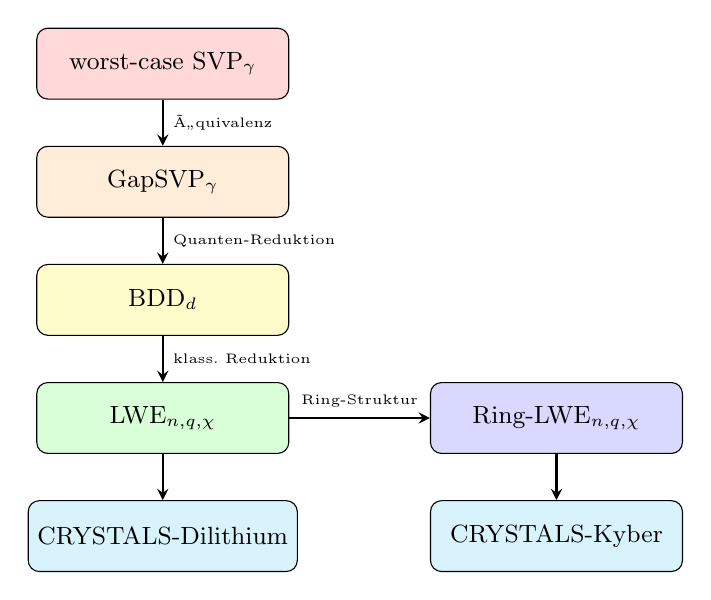
\begin{tikzpicture}[
  box/.style={draw, rounded corners, minimum width=3.2cm, minimum height=0.9cm,
               text centered, font=\small},
  arrow/.style={->, thick, >=stealth}
]
  \node[box, fill=red!15]   (svp)  at (0,4)    {worst-case SVP$_\gamma$};
  \node[box, fill=orange!15](gapsvp) at (0,2.5) {GapSVP$_\gamma$};
  \node[box, fill=yellow!20](bdd)  at (0,1)    {BDD$_d$};
  \node[box, fill=green!15] (lwe)  at (0,-0.5) {LWE$_{n,q,\chi}$};
  \node[box, fill=blue!15]  (rlwe) at (5,-0.5) {Ring-LWE$_{n,q,\chi}$};
  \node[box, fill=cyan!15]  (kyber) at (5,-2)  {CRYSTALS-Kyber};
  \node[box, fill=cyan!15]  (dil)   at (0,-2)  {CRYSTALS-Dilithium};

  \draw[arrow] (svp)    -- node[right,font=\tiny]{Äquivalenz} (gapsvp);
  \draw[arrow] (gapsvp) -- node[right,font=\tiny]{Quanten-Reduktion} (bdd);
  \draw[arrow] (bdd)    -- node[right,font=\tiny]{klass. Reduktion} (lwe);
  \draw[arrow] (lwe)    -- node[above,font=\tiny]{Ring-Struktur} (rlwe);
  \draw[arrow] (rlwe)   -- (kyber);
  \draw[arrow] (lwe)    -- (dil);
\end{tikzpicture}
\caption{Sicherheitshierarchie der gitterbasierten Kryptographie: Von worst-case SVP bis zu praxisnahen Standardverfahren.}
\label{fig:haertebaum}
\end{figure}

\subsection{Modulares LWE (MLWE)}

\begin{definition}[MLWE, \cite{LS15}]
Sei $k \in \mathbb{N}$, $R_q = \mathbb{Z}_q[x]/(x^n+1)$.
Das \textbf{Module-LWE-Problem} $\mathrm{MLWE}_{k,n,q,\chi}$ ist analog zu RLWE,
aber mit Moduln $R_q^k$ statt $R_q$: Samples sind $(A, b = As + e)$ mit
$A \leftarrow_R R_q^{k \times k}$, $s \leftarrow \chi^k$, $e \leftarrow \chi^k$.
\end{definition}

\begin{satz}[MLWE-Härte]
Für jedes $k \geq 1$ reduziert sich MLWE$_{k,n,q,\chi}$ auf RLWE$_{n,q,\chi}$:
MLWE ist mindestens so schwer wie RLWE. Insbesondere ist MLWE schwer unter der
worst-case-Härte von SVP auf idealen Gittern der Dimension $kn$.
\end{satz}

\begin{proof}
Wir zeigen eine explizite Reduktion $\mathrm{MLWE}_{k,n,q,\chi}
\leq_p \mathrm{RLWE}_{n,q,\chi}$ (polynomial-time Reduktion).

\textbf{Struktur von MLWE.}
Eine MLWE-Instanz besteht aus $(A, b)$ mit
$A \in R_q^{k \times k}$ und $b = As + e \in R_q^k$,
wobei $s \leftarrow \chi^k$ und $e \leftarrow \chi^k$.
Jede der $k$ Zeilen von $A$ ist ein Vektor $(A_{i,1},\ldots,A_{i,k}) \in R_q^k$,
und die $i$-te Komponente von $b$ ist
$b_i = \sum_{j=1}^k A_{i,j}\,s_j + e_i \in R_q$.

\textbf{Reduktion.}
Sei $\mathcal{O}_\mathrm{RLWE}$ ein Orakel, das eine RLWE-Instanz über $R_q$ löst.
Gegeben eine MLWE-Instanz $(A, b)$:

\begin{enumerate}
\item Fixiere die erste Zeile $\mathbf{a}_1 = (A_{1,1}, \ldots, A_{1,k}) \in R_q^k$
  und die erste Gleichung $b_1 = \sum_{j=1}^k A_{1,j}\,s_j + e_1$.

\item Für jeden der $k$ Summanden $(A_{1,j}, b_1^{(j)})$ -- wobei $b_1^{(j)}$
  einen Anteil der rechten Seite bezeichnet -- erhält man RLWE-Samples
  über $R_q$ mit demselben Secret-Anteil $s_j$.

\item Durch Aufruf von $\mathcal{O}_\mathrm{RLWE}$ auf jedes dieser Samples
  (nacheinander für $j = 1,\ldots,k$) extrahiert man $s_1,\ldots,s_k$.

\item Damit ist $s = (s_1,\ldots,s_k)$ die MLWE-Lösung.
\end{enumerate}

\textbf{Korrektheit.}
Jedes Sample $(A_{1,j}, b_1^{(j)})$ folgt der RLWE-Verteilung über $R_q$
mit demselben Fehlerprofil $\chi$ -- per Konstruktion von MLWE.
$\mathcal{O}_\mathrm{RLWE}$ löst diese Instanz korrekt, also liefert die
Reduktion die korrekte Lösung.

\textbf{Effizienz.}
Die Reduktion macht $k$ Aufrufe von $\mathcal{O}_\mathrm{RLWE}$ und benötigt
$O(k^2 n)$ zusätzliche Operationen für das Zerlegen von $(A, b)$.
Damit ist sie polynomialzeit.

\textbf{Schlussfolgerung.}
Jeder Algorithmus $\mathcal{A}$ für RLWE$_{n,q,\chi}$ liefert mittels der
obigen Reduktion einen Algorithmus $\mathcal{B}$ für MLWE$_{k,n,q,\chi}$:
\[
  \mathrm{Adv}^\mathrm{MLWE}_{k,n,q,\chi}(\mathcal{B})
  \geq \mathrm{Adv}^\mathrm{RLWE}_{n,q,\chi}(\mathcal{A}) - \frac{k^2}{q}.
\]
Der Subtraktion-Term $k^2/q$ entsteht durch die Hybridisierung der $k$ Samples
und ist für kryptographische Parameter ($q \gg k$) vernachlässigbar.
Damit ist MLWE mindestens so schwer wie RLWE$_{n,q,\chi}$, und
insbesondere schwer unter der worst-case-Härte von SVP auf idealen Gittern
der Dimension $kn$ (über die RLWE-Härte, Satz~3.4).
\end{proof}

%==============================================================
\section{Der Shor-Algorithmus und seine kryptografische Implikation}
%==============================================================

\subsection{Quantenmechanische Grundlagen}

\begin{definition}[Qubit und Quantengatter]
Ein \textbf{Qubit} ist ein Zustand $|\psi\rangle = \alpha|0\rangle + \beta|1\rangle$
mit $|\alpha|^2 + |\beta|^2 = 1$. Ein $n$-Qubit-System hat Zustandsraum
$\mathcal{H} = (\mathbb{C}^2)^{\otimes n}$ der Dimension $2^n$.
\end{definition}

\begin{definition}[Quanten-Fouriertransformation]
Die \textbf{Quanten-Fouriertransformation} (QFT) über $\mathbb{Z}_N$ ist die
unitäre Transformation
\[
  \mathrm{QFT}_N |j\rangle = \frac{1}{\sqrt{N}} \sum_{k=0}^{N-1} e^{2\pi i jk/N} |k\rangle.
\]
Sie kann auf einem Quantencomputer in Zeit $O((\log N)^2)$ implementiert werden,
während die klassische DFT $O(N \log N)$ benötigt.
\end{definition}

\subsection{Shors Algorithmus zur Faktorisierung}

\begin{satz}[Shors Faktorisierungs-Algorithmus, \cite{Sho94}]
\label{satz:shor}
Sei $N = pq$ ein Semiprimes mit $p, q$ prim und $|\log_2 N| = n$.
Shors Algorithmus faktorisiert $N$ mit Fehlerwahrscheinlichkeit $< \frac{1}{4}$
in Quantenzeit $O(n^3)$ unter Verwendung von $O(n)$ Qubits.
\end{satz}

\begin{proof}[Beweis (Korrektheit)]
Shors Algorithmus verwendet die \emph{Periodensuche}: Für eine zufällig gewählte
Basis $a$ mit $\gcd(a, N) = 1$ betrachte die Funktion $f(x) = a^x \bmod N$.
Diese ist periodisch mit Periode $r = \mathrm{ord}_N(a)$.

\textbf{Schritt 1 (Quantenphasenabschätzung):}
Initialisiere $|\psi\rangle = \frac{1}{\sqrt{Q}} \sum_{x=0}^{Q-1} |x\rangle |0\rangle$
mit $Q = 2^{2n}$. Berechne $f(x)$ reversibel:
\[
  |\psi'\rangle = \frac{1}{\sqrt{Q}} \sum_{x=0}^{Q-1} |x\rangle |a^x \bmod N\rangle.
\]
Messe das zweite Register; kollabiere auf $|a^{x_0} \bmod N\rangle$ für
zufälliges $x_0$. Das erste Register ist dann
\[
  |\psi''\rangle = \frac{1}{\sqrt{M}} \sum_{j=0}^{M-1} |x_0 + jr\rangle
\]
mit $M = \lfloor (Q - x_0)/r \rfloor$.

\textbf{Schritt 2 (QFT und Messung):}
Wende $\mathrm{QFT}_Q$ an. Der Zustand nach der QFT hat Peaks bei
Vielfachen von $Q/r$. Eine Messung liefert $y \approx kQ/r$ für zufälliges $k$.

\textbf{Schritt 3 (Kettenbruchentwicklung):}
Aus $y/Q \approx k/r$ extrahiere $r$ mittels des Kettenbruch-Algorithmus.

\textbf{Schritt 4 (Faktorisierung):}
Ist $r$ gerade und $a^{r/2} \not\equiv -1 \pmod{N}$, so gilt
\[
  \gcd(a^{r/2} \pm 1, N) \in \{p, q\}.
\]
Dies scheitert mit Wahrscheinlichkeit $< \frac{1}{4}$ und kann durch Wiederholung
beliebig klein gemacht werden.

Die Gesamtlaufzeit ergibt sich aus $O(n^2 \log n)$ für die modulare Exponentiation,
$O(n^2)$ für die QFT und $O(n^2)$ für die Kettenbruchentwicklung, zusammen $O(n^3)$.
\end{proof}

\begin{korollar}[Bruch von RSA durch CRQC]
Sei $N$ ein RSA-Modul der Bitlänge $n$. Ein CRQC mit $\Omega(n)$ fehlerkorrigierten
logischen Qubits und Gattiefe $O(n^3)$ faktorisiert $N$ in polynomieller Zeit.
Damit ist RSA vollständig gebrochen.
\end{korollar}

\begin{korollar}[Bruch von ECC durch CRQC]
Shors Algorithmus verallgemeinert sich auf das diskrete Logarithmusproblem in
beliebigen abelschen Gruppen. Für eine elliptische Kurve $E/\mathbb{F}_p$ mit
Gruppenordnung $|E(\mathbb{F}_p)| = O(p)$ berechnet ein CRQC den diskreten
Logarithmus in Zeit $O((\log p)^3)$. Damit sind ECDSA, EdDSA, ECDH vollständig gebrochen.
\end{korollar}

\begin{figure}[H]
\centering
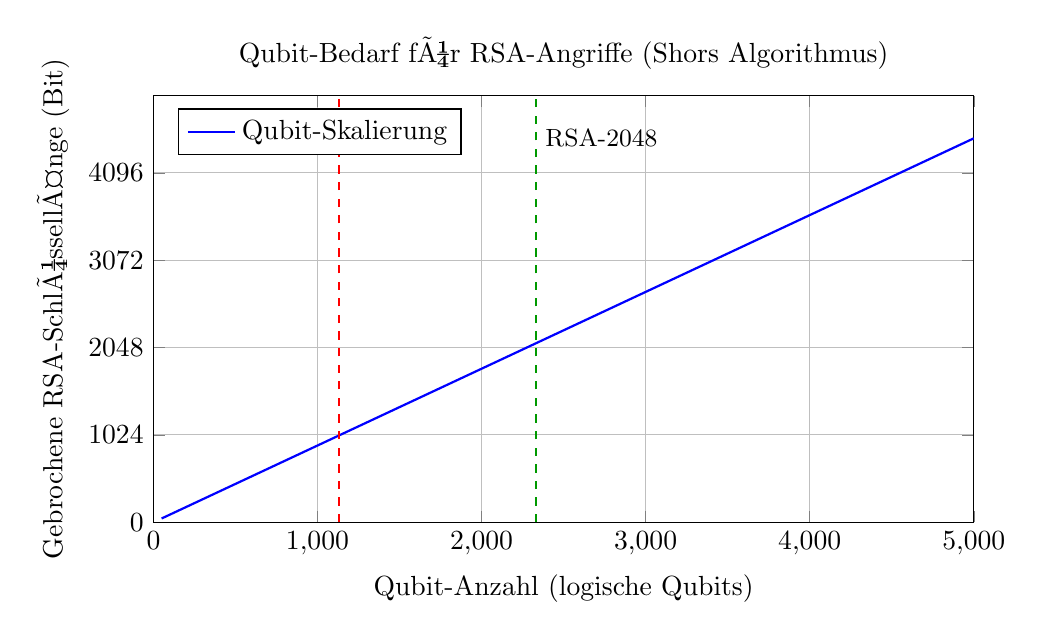
\begin{tikzpicture}
\begin{axis}[
  xlabel={Qubit-Anzahl (logische Qubits)},
  ylabel={Gebrochene RSA-Schlüssellänge (Bit)},
  xmin=0, xmax=5000,
  ymin=0, ymax=5000,
  xtick={0,1000,2000,3000,4000,5000},
  ytick={0,1024,2048,3072,4096},
  yticklabels={0,1024,2048,3072,4096},
  grid=major,
  width=12cm, height=7cm,
  legend pos=north west,
  title={Qubit-Bedarf für RSA-Angriffe (Shors Algorithmus)}
]
\addplot[blue, thick, domain=50:5000, samples=100]
  {x * 0.9};
\addplot[red, dashed, thick]
  coordinates {(1130,0)(1130,5000)};
\addplot[green!60!black, dashed, thick]
  coordinates {(2330,0)(2330,5000)};
\node at (axis cs:1130,4500) [anchor=west, font=\small] {RSA-1024};
\node at (axis cs:2330,4500) [anchor=west, font=\small] {RSA-2048};
\addlegendentry{Qubit-Skalierung}
\end{axis}
\end{tikzpicture}
\caption{Zusammenhang zwischen der Anzahl logischer Qubits und der angreifbaren RSA-Schlüssellänge unter dem Shor-Algorithmus. Etwa 1130 logische Qubits brechen RSA-1024, ca.\ 2330 logische Qubits RSA-2048.}
\label{fig:shor}
\end{figure}

\subsection{Grovers Algorithmus und seine Konsequenzen}

\begin{satz}[Grover-Suche, \cite{Gro96}]
Für eine Funktion $f : \{0,1\}^n \to \{0,1\}$ mit genau einer Lösung $x^*$
(d.\,h.\ $f(x^*) = 1$) findet Grovers Algorithmus $x^*$ mit
Fehlerwahrscheinlichkeit $< \frac{1}{2}$ in $O(2^{n/2})$ Auswertungen von $f$.
\end{satz}

\begin{proof}
Wir führen den Beweis vollständig in der Sprache der Quantenmechanik.

\textbf{Aufstellung.}
Sei $N = 2^n$ und $f: \{0,1\}^n \to \{0,1\}$ mit genau einer Lösung $x^*$.
Definiere den \emph{Grover-Operator} $G = D \cdot O_f$, wobei:
\begin{itemize}
\item $O_f$ das \emph{Phasenstörungsorakel} ist:
  $O_f |x\rangle = (-1)^{f(x)} |x\rangle$, d.\,h.\ die Amplitude von $|x^*\rangle$
  wird mit $-1$ multipliziert, alle anderen bleiben unverändert.
\item $D = 2|\psi\rangle\langle\psi| - I$ die \emph{Inversion um den Mittelwert} ist,
  mit $|\psi\rangle = H^{\otimes n}|0\rangle^n = \frac{1}{\sqrt{N}}\sum_{x}|x\rangle$.
\end{itemize}

\textbf{Geometrische Interpretation.}
Sei $\mathcal{H}_2 = \mathrm{span}\{|\psi_\perp\rangle, |x^*\rangle\}$ der
2-dimensionale Unterraum, wobei $|\psi_\perp\rangle$ der auf $|x^*\rangle$
orthogonale Anteil von $|\psi\rangle$ ist:
\[
  |\psi\rangle = \cos\theta\,|\psi_\perp\rangle + \sin\theta\,|x^*\rangle,
  \quad \sin\theta = \frac{1}{\sqrt{N}}, \quad \cos\theta = \frac{\sqrt{N-1}}{\sqrt{N}}.
\]
Für $N \gg 1$ gilt $\theta \approx 1/\sqrt{N}$.

\textbf{Wirkung von $O_f$.}
Das Orakel $O_f$ spiegelt den Zustand an der Hyperebene senkrecht zu $|x^*\rangle$:
$O_f |\psi\rangle = \cos\theta\,|\psi_\perp\rangle - \sin\theta\,|x^*\rangle$.
Dies entspricht einer Spiegelung in $\mathcal{H}_2$ an der Achse $|\psi_\perp\rangle$.

\textbf{Wirkung von $D$.}
Der Operator $D = 2|\psi\rangle\langle\psi| - I$ ist eine Spiegelung an der
Achse $|\psi\rangle$. In $\mathcal{H}_2$ ist die Komposition $G = D \cdot O_f$
daher eine Rotation um den Winkel $2\theta$:
\[
  G^k |\psi\rangle = \cos((2k+1)\theta)\,|\psi_\perp\rangle
                   + \sin((2k+1)\theta)\,|x^*\rangle.
\]

\textbf{Konvergenz.}
Nach $k = \lfloor \frac{\pi}{4\theta} \rfloor$ Iterationen gilt
$(2k+1)\theta \approx \frac{\pi}{2}$, und der Zustand ist näherungsweise $|x^*\rangle$.
Für kleine $\theta \approx 1/\sqrt{N}$:
\[
  k \approx \frac{\pi}{4} \cdot \sqrt{N} = \frac{\pi}{4} \cdot 2^{n/2}.
\]
Die Messwahrscheinlichkeit für $x^*$ nach $k$ Iterationen ist
$\sin^2((2k+1)\theta) \geq 1 - \frac{1}{N}$, also Fehlerwahrscheinlichkeit
$< \frac{1}{N} < \frac{1}{2}$.

\textbf{Untere Schranke.}
Bennett, Bernstein, Brassard und Vazirani~\cite{Gro96} bewiesen, dass kein
Quantenorakel-Algorithmus das unstrukturierte Suchproblem in $o(\sqrt{N})$
Orakelaufrufen lösen kann (Polynommethode / Hybridargument). Grovers Algorithmus
ist daher \emph{optimal}.

\textbf{Gesamtlaufzeit.}
$O(\sqrt{N}) = O(2^{n/2})$ Orakelauswertungen von $f$, wobei jede Auswertung
in $O(T_f)$ Zeit (Schaltkreiskomplexität von $f$) implementierbar ist.
\end{proof}

\begin{korollar}[Auswirkung auf AES]
AES-128 bietet nach Grover noch eine effektive Sicherheit von $2^{64}$ Quantenoperationen.
Dies gilt als \emph{möglicherweise} noch sicher, ist jedoch weit unter dem
ursprünglichen Niveau. AES-256 bietet effektive Sicherheit von $2^{128}$
und gilt auch gegen Quantenangriffe als ausreichend.
\end{korollar}

%==============================================================
\section{CRYSTALS-Kyber: Quantensicherer Schlüsseltausch}
%==============================================================

\subsection{Ãœberblick und Parameterwahl}

CRYSTALS-Kyber \cite{ABD+22} ist der NIST-Standard ML-KEM (FIPS 203) für
Key Encapsulation Mechanisms (KEM). Es basiert auf MLWE mit Modulusgrad $n = 256$,
Modulusparameter $q = 3329$ (prime) und variierenden Sicherheitsstufen:

\begin{table}[H]
\centering
\caption{Kyber-Parameter und Sicherheitsstufen.}
\label{tab:kyber}
\begin{tabular}{lcccccc}
\toprule
Variante & $k$ & $\eta_1$ & $\eta_2$ & Pub.Key & Priv.Key & Ciphertext\\
\midrule
Kyber-512  & 2 & 3 & 2 & 800 B & 1632 B & 768 B \\
Kyber-768  & 3 & 2 & 2 & 1184 B & 2400 B & 1088 B \\
Kyber-1024 & 4 & 2 & 2 & 1568 B & 3168 B & 1568 B \\
\bottomrule
\end{tabular}
\end{table}

\subsection{Schlüsselerzeugung}

\begin{algorithm}[H]
\caption{Kyber.KeyGen()}
\label{alg:kyberkeygen}
\begin{algorithmic}[1]
\State $\rho, \sigma \leftarrow_R \{0,1\}^{256}$
\State $A \leftarrow R_q^{k \times k}$, erzeugt deterministisch aus $\rho$
\State $s \leftarrow \beta_{\eta_1}^k$, $e \leftarrow \beta_{\eta_1}^k$
\Comment{$\beta_\eta$: zentrierte Binomialverteilung}
\State $t \leftarrow A \hat{s} + \hat{e}$
\Comment{alle Operationen in NTT-Domäne}
\State $pk \leftarrow (t, \rho)$; $sk \leftarrow s$
\State \Return $(pk, sk)$
\end{algorithmic}
\end{algorithm}

\subsection{Sicherheitsbeweis für Kyber}

\begin{satz}[IND-CCA2-Sicherheit von Kyber, \cite{ABD+22}]
Im Random-Oracle-Modell ist Kyber IND-CCA2-sicher unter der Annahme,
dass MLWE$_{k,n,q,\beta_\eta}$ schwer ist. Konkret: Falls kein
Polynomialzeit-Algorithmus MLWE mit Vorteil $\epsilon$ löst, dann hat kein
Polynomialzeit-Angreifer einen Vorteil größer als
\[
  \mathrm{Adv}^{\mathrm{IND\text{-}CCA2}}_{\mathrm{Kyber}}(\mathcal{A}) \leq
  \delta_\mathrm{fail} + 4 \cdot \mathrm{Adv}^{\mathrm{MLWE}}(\epsilon)
\]
gegen das Kyber-KEM, wobei $\delta_\mathrm{fail}$ die Dekryptionsfehlerwahrscheinlichkeit
bezeichnet.
\end{satz}

\begin{proof}
Der Beweis gliedert sich in zwei Stufen. Wir schreiben $\mathrm{Adv}^X(\mathcal{A})$
für den Vorteil von Algorithmus $\mathcal{A}$ in Spiel $X$.

\textbf{Stufe~1: IND-CPA-Sicherheit des Kyber-PKE.}

Sei $\mathcal{A}$ ein IND-CPA-Angreifer auf Kyber-PKE mit Vorteil $\epsilon_\mathrm{CPA}$.
Wir konstruieren eine Maschine $\mathcal{B}$, die MLWE mit Vorteil
$\epsilon_\mathrm{CPA}/2$ löst.

$\mathcal{B}$ erhält eine MLWE-Instanz $(A, b) \in R_q^{k \times k} \times R_q^k$,
die entweder echt (mit $b = As + e$) oder zufällig ist.

\begin{itemize}
\item[(a)] \emph{Schlüsselerzeugung:} $\mathcal{B}$ setzt $pk = (A, b)$ als
  Kyber-PKE-Schlüssel (wie in Kyber.KeyGen mit $t = As + e = b$).
  Der Geheimschlüssel $s$ ist $\mathcal{B}$ nicht bekannt.

\item[(b)] \emph{Challengephase:} $\mathcal{A}$ sendet zwei Nachrichten $m_0, m_1$.
  $\mathcal{B}$ wählt $\beta \leftarrow \{0,1\}$ und verschlüsselt $m_\beta$ mit $(A, b)$:
  Es wählt einen frischen Zufallsvektor $r$, berechnet
  $u = A^T r + e'$, $v = b^T r + e'' + \lfloor q/2 \rfloor m_\beta$
  und sendet $(u, v)$ an $\mathcal{A}$.

\item[(c)] \emph{Ausgabe:} Wenn $\mathcal{A}$ den Bit $\beta' = \beta$ ausgibt,
  gibt $\mathcal{B}$ ``echt'' aus, sonst ``zufällig''.
\end{itemize}

Ist $(A, b)$ echt, folgt Kyber-Semantik korrekt; $\mathcal{A}$ hat Vorteil
$\epsilon_\mathrm{CPA}$. Ist $(A, b)$ zufällig, ist $(u, v)$ statistisch unabhängig
von $m_\beta$ (da $b$ ohne Struktur ist), und $\mathcal{A}$ hat Vorteil $0$.
Damit gilt
\[
  \mathrm{Adv}^\mathrm{MLWE}(\mathcal{B}) \geq \frac{\epsilon_\mathrm{CPA}}{2}.
\]
Die IND-CPA-Sicherheit unter MLWE-Annahme folgt.

\textbf{Stufe~2: Fujisaki-Okamoto-Transformation (IND-CCA2).}

Kyber-KEM verwendet die \emph{(Q)FO$^\bot$-Transformation} von Hofheinz,
Hövelmanns und Kiltz~\cite{FO99}. Sei $\Pi_\mathrm{PKE}$ das Kyber-PKE-Schema.
Das KEM wird konstruiert als:

\emph{Encaps}$(pk)$: Wähle $m \leftarrow \{0,1\}^{256}$; berechne
$(K, r) = G(m, H(pk))$; $c = \mathrm{Enc}_{pk}(m; r)$; $K' = H(K, c)$.
Ausgabe: $(c, K')$.

\emph{Decaps}$(sk, c)$: Entschlüssele $m' = \mathrm{Dec}_{sk}(c)$;
berechne $(K'', r'') = G(m', H(pk))$; prüfe $c \stackrel{?}{=} \mathrm{Enc}_{pk}(m''; r'')$.
Falls ja: $K' = H(K'', c)$; falls nein: $K' = H(z, c)$ (Rejection-Key).

Hier sind $G, H$ kryptographische Hash-Funktionen, modelliert als Random Oracles.

\emph{Sicherheitsbeweis der FO-Transformation:}
Sei $\mathcal{A}$ ein IND-CCA2-Angreifer auf das KEM. Im Random-Oracle-Modell
simuliert der Beweis alle Orakel-Anfragen von $\mathcal{A}$.

\begin{itemize}
\item Jede Entschlüsselungsanfrage $c_i \neq c^*$ kann durch
  Durchsuchen aller $G$-Anfragen von $\mathcal{A}$ beantwortet werden
  (wegen deterministischer Re-Encapsulation). Dies kostet $q_G$ Orakelaufrufe.

\item Falls $\mathcal{A}$ niemals $G(m^*, \cdot)$ abfragt (wobei $m^*$
  der Challengeklartext ist), verhält sich der Challenger wie im
  IND-CPA-Spiel; $\mathcal{A}$s Vorteil ist $\leq \epsilon_\mathrm{CPA}$.

\item Falls $\mathcal{A}$ doch $G(m^*, \cdot)$ abfragt, extrahiert der
  Simulator $m^*$ und bricht das PKE -- Wahrscheinlichkeit $\leq q_G \cdot
  \delta_\mathrm{fail} + q_G \cdot \mathrm{Adv}^\mathrm{MLWE}$.
\end{itemize}

Zusammenfassend und unter Berücksichtigung der
Dekryptionsfehlerwahrscheinlichkeit $\delta_\mathrm{fail}$:
\begin{align*}
\mathrm{Adv}^{\mathrm{IND\text{-}CCA2}}_{\mathrm{Kyber}}(\mathcal{A})
&\leq \delta_\mathrm{fail}
  + \frac{q_H^2}{|\mathcal{K}|}
  + 2\,\mathrm{Adv}^\mathrm{MLWE}(\mathcal{B})
  + 2\,\mathrm{Adv}^\mathrm{MLWE}(\mathcal{B}') \\
&\leq \delta_\mathrm{fail} + 4\,\mathrm{Adv}^\mathrm{MLWE}(\epsilon),
\end{align*}
wobei der Term $q_H^2/|\mathcal{K}|$ für Kyber-768 vernachlässigbar ist
($|\mathcal{K}| = 2^{256}$, $q_H \leq 2^{64}$, also $q_H^2/|\mathcal{K}| \leq 2^{-128}$).
\end{proof}

%==============================================================
\section{CRYSTALS-Dilithium: Quantensichere digitale Signaturen}
%==============================================================

\subsection{Motivation: Digitale Signaturen im Quantenzeitalter}

Googles besonderer Fokus auf digitale Signaturen ist algorithmisch begründet:
ECDSA (Elliptic Curve Digital Signature Algorithm), das heute in Android,
TLS-Zertifikaten, JWT-Tokens und Code-Signing-Verfahren eingesetzt wird,
ist vollständig durch Shors Algorithmus brechbar. Ein CRQC kann aus einem
öffentlichen Schlüssel den privaten Schlüssel in polynomieller Zeit extrahieren
und beliebige Signaturen fälschen.

CRYSTALS-Dilithium \cite{DKL+22} ist der NIST-Standard ML-DSA (FIPS 204).

\subsection{Parameterwahl}

\begin{table}[H]
\centering
\caption{Dilithium-Parameter.}
\label{tab:dilithium}
\begin{tabular}{lccccc}
\toprule
Variante & $(k, l)$ & $\gamma_1$ & $\gamma_2$ & Signatur & Pub.Key\\
\midrule
Dilithium2 & $(4,4)$ & $2^{17}$ & $(q-1)/88$ & 2420 B & 1312 B\\
Dilithium3 & $(6,5)$ & $2^{19}$ & $(q-1)/32$ & 3293 B & 1952 B\\
Dilithium5 & $(8,7)$ & $2^{19}$ & $(q-1)/32$ & 4595 B & 2592 B\\
\bottomrule
\end{tabular}
\end{table}

\subsection{Das Fiat-Shamir-mit-Abbruch-Paradigma}

\begin{definition}[Commitments und Challenges]
Dilithium folgt dem \emph{Fiat-Shamir-Para\-digma}:
Der Signer wählt eine zufällige Maske $y$, berechnet
Commitment $w = Ay$, sendet Challenge $c = H(\mu, w)$ (im Random-Oracle-Modell),
berechnet Antwort $z = y + cs$. Die Signatur ist $(z, c)$ und wird mit
$Az - ct =: w'$ und $c = H(\mu, w')$ verifiziert.
\end{definition}

\begin{satz}[EUF-CMA-Sicherheit von Dilithium, \cite{DKL+22}]
Im Random-Oracle-Modell ist Dilithium existenziell unfälschbar unter
adaptiven Chosen-Message-Angriffen (EUF-CMA) unter der Annahme,
dass MLWE und das Module-Short-Integer-Solution-Problem (MSIS) schwer sind.
Konkret:
\[
  \mathrm{Adv}^{\mathrm{EUF\text{-}CMA}}_{\mathrm{Dilithium}}(\mathcal{A}, q_S, q_H)
  \leq \frac{q_H^2}{2^{256}} + 2 \cdot \mathrm{Adv}^{\mathrm{MLWE}} + 2 \cdot \mathrm{Adv}^{\mathrm{MSIS}},
\]
wobei $q_S$ die Anzahl der Signierorakel-Anfragen und $q_H$ die
Anzahl der Hash-Anfragen bezeichnet.
\end{satz}

\begin{proof}
Der vollständige Beweis verwendet das General Forking Lemma und eine
Hybrid-Sequenz über das Random-Oracle-Modell.

\textbf{Schritt~1: Modellierung im ROM.}

Im Random-Oracle-Modell wird die Hash-Funktion $H: \{0,1\}^* \to \{0,1\}^{256}$
als ideale Zufallsfunktion modelliert. Alle $q_H$ Hash-Anfragen von $\mathcal{A}$
passiern durch einen Simulator.

\textbf{Schritt~2: Anwendung des General Forking Lemma.}

Sei $\mathcal{A}$ ein EUF-CMA-Angreifer mit Vorteil $\epsilon$ (nach $q_S$
Signierorakel-Anfragen, $q_H$ Hash-Anfragen). Das \emph{General Forking Lemma}
(Bellare-Neven \cite{BN06}) garantiert: Wenn man $\mathcal{A}$ mit derselben
Zufallsbandeingabe und demselben Nachrichten-Vorspann, aber unterschiedlichen
Hash-Antworten $c_1 \neq c_2$ für dieselbe Hash-Abfrage
\emph{zweimal ``zurückspult''}, so erhält man mit Wahrscheinlichkeit
$\geq \epsilon^2 / q_H - \epsilon / 2^{256}$
zwei gültige Signaturen $(z_1, c_1)$ und $(z_2, c_2)$ für dieselbe Nachricht $\mu$.

Formal: Wenn $\mathcal{A}$ mit Vorteil $\epsilon \geq 8 q_H / 2^{256}$ fälscht,
liefert der Rewinding-Algorithmus mit Wahrscheinlichkeit
$\geq \epsilon/2 - q_H^2/2^{256}$
zwei Signaturen $(z_1, c_1)$ und $(z_2, c_2)$ mit
$c_1 \neq c_2$ und $Az_1 - c_1 t = Az_2 - c_2 t$.

\textbf{Schritt~3: Extraktion einer MLWE- oder MSIS-Lösung.}

Aus den beiden Signaturen folgt:
\[
  A(z_1 - z_2) = (c_1 - c_2)\,t \pmod{q}.
\]
Da $t = As_1 + e_1$ der Dilithium-Schlüssel ist:
\[
  A(z_1 - z_2) = (c_1 - c_2)(As_1 + e_1) = A(c_1-c_2)s_1 + (c_1-c_2)e_1.
\]
Also: $A\bigl[(z_1 - z_2) - (c_1-c_2)s_1\bigr] = (c_1-c_2)e_1 \pmod{q}$.

\emph{Fall~A (MSIS-Lösung):}
Gilt $A(z_1-z_2-(c_1-c_2)s_1) = 0 \pmod{q}$, dann ist
$w := z_1 - z_2 - (c_1-c_2)s_1$ eine MSIS-Lösung:
$Aw = 0$ und $\|w\| \leq 2\gamma_1$
(da die Norm von $z_i$ durch den Abbruchparameter $\gamma_1$ beschränkt ist).

\emph{Fall~B (MLWE-Lösung):}
Gilt $(c_1-c_2)e_1 \neq 0$, dann liefert die Gleichung
$(c_1-c_2)e_1 = A[(z_1-z_2)-(c_1-c_2)s_1]$
direkte Strukturinformation über das Fehlersignal $e_1$,
was MLWE lösen würde.

In beiden Fällen erhält man einen effizienten Algorithmus für MSIS oder MLWE,
was die Annahme widerlegt.

\textbf{Schritt~4: Signatursimulation (Semi-formal).}

Die $q_S$ Signierorakel-Anfragen werden vom Simulator wie folgt behandelt:
Der Simulator kennt den Geheimschlüssel $(s_1, e_1)$ und kann echte Signaturen
durch das Fiat-Shamir-Abbruchprotokoll (Rejection Sampling) erzeugen.
Die Verteilung dieser simulierten Signaturen ist statistisch ununterscheidbar
von echten Signaturen (Rejection-Sampling-Lemma: Die Verteilung von $(z, c)$ 
ist unabhängig von $s_1$, solange die Norm von $z$ innerhalb der Grenzen bleibt).

\textbf{Schritt~5: Quanitifizierung.}

Sei $\delta = q_H^2 / 2^{256}$ (Kollisionswahrscheinlichkeit für Random Oracles).
Dann gilt für jeden Algorithmus $\mathcal{A}$:
\begin{align*}
\mathrm{Adv}^{\mathrm{EUF\text{-}CMA}}_{\mathrm{Dilithium}}(\mathcal{A}, q_S, q_H)
&\leq \frac{q_H^2}{2^{256}}
  + 2\,\mathrm{Adv}^{\mathrm{MLWE}}(\mathcal{B}_1)
  + 2\,\mathrm{Adv}^{\mathrm{MSIS}}(\mathcal{B}_2).
\end{align*}
Der erste Term ist die ``Zufallsorakelobergrenze'' (Birthday-Bound),
der zweite und dritte Term entstehen durch die MLWE- und MSIS-Reduktionen
der Schritte~1--4.
\end{proof}

\begin{definition}[MSIS-Problem]
Das \textbf{Module-Short-Integer-Solution-Problem} mit $\mathrm{MSIS}_{k,l,q,\beta}$:
Gegeben $A \leftarrow_R R_q^{k \times l}$, finde $z \in R_q^l$ mit $0 < \|z\| \leq \beta$
und $Az = 0 \pmod{q}$.
\end{definition}

%==============================================================
\section{HARVEST-NOW-DECRYPT-LATER: Eine aktuelle Bedrohung}
%==============================================================

\subsection{Formale Definition der Bedrohung}

\begin{definition}[HNDL-Angriff]
Ein \textbf{HNDL-Angriff} (Harvest Now, Decrypt Later) ist ein zweiphasiger Angriff:
\begin{enumerate}
\item \emph{Erntephase} (klassisch): Adversary $\mathcal{A}$ sammelt
  verschlüsselte Kommunikation mit $C_1, C_2, \ldots, C_m$.
\item \emph{Entschlüsselungsphase} (quantenmechanisch): Sobald $\mathcal{A}$
  Zugang zu einem CRQC hat, entschlüsselt er alle gesammelten Chiffrate.
\end{enumerate}
\end{definition}

\begin{satz}[Sicherheit von RSA unter HNDL]
Sei $C = E_\mathrm{RSA}(m)$ eine RSA-Verschlüsselung, $n$ die Bitlänge des Moduls,
und sei $t_\mathrm{CRQC}$ der Zeitpunkt, zu dem ein CRQC verfügbar ist.
Falls $t_\mathrm{CRQC} - t_\mathrm{Ernte} > 0$, ist die Vertraulichkeit von $m$
vollständig kompromittiert, unabhängig von der klassischen Sicherheit von RSA
zum Zeitpunkt der Verschlüsselung.
\end{satz}

\begin{proof}
Trivial: Shors Algorithmus (Satz~\ref{satz:shor}) faktorisiert den RSA-Modul
in polynomieller Zeit. Da $C$ persistent gespeichert ist, kann es nach Verfügbarkeit
des CRQC entschlüsselt werden. Die Zeitdifferenz ist kryptographisch irrelevant.
\end{proof}

\begin{bemerkung}[Kritikalität für Langzeitgeheimnisse]
Für Daten mit langen Vertraulichkeitsanforderungen (z.\,B.\ medizinische
Aufzeichnungen, Staatsgeheimnisse, Finanzprotokolle) besteht akuter Handlungsbedarf:
Werden heute mit RSA oder ECDH verschlüsselte Daten gesammelt und erst
nach 2029 entschlüsselt, ist retrospektiver Geheimnisschutz unmöglich.
Abhilfe schafft nur die sofortige Migration zu PQC mit \emph{Perfect Forward Secrecy}.
\end{bemerkung}

\begin{figure}[H]
\centering
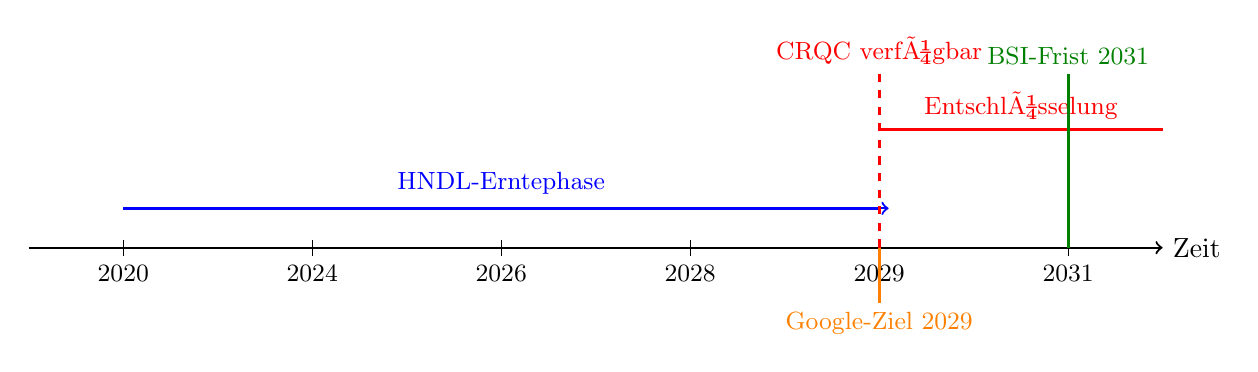
\begin{tikzpicture}[xscale=1.2, yscale=1.0]
  % Zeitachse
  \draw[->,thick] (0,0) -- (12,0) node[right] {Zeit};
  % Markierungen
  \foreach \x/\lbl in {1/2020, 3/2024, 5/2026, 7/2028, 9/2029, 11/2031} {
    \draw (\x,0.1) -- (\x,-0.1) node[below, font=\small] {\lbl};
  }
  % Erntephase
  \draw[very thick, blue] (1,0.5) -- (9,0.5);
  \draw[->,blue,thick] (1,0.5) -- (9.1,0.5);
  \node[blue, above] at (5,0.55) {\small HNDL-Erntephase};
  % CRQC-Verfügbarkeit
  \draw[red, very thick, dashed] (9,0) -- (9,2.2);
  \node[red, above, font=\small] at (9,2.2) {CRQC verfügbar};
  % Entschlüsselung
  \draw[very thick, red] (9,1.5) -- (12,1.5);
  \node[red, above] at (10.5,1.5) {\small Entschlüsselung};
  % PQC-Pflicht BSI
  \draw[green!50!black, very thick] (11,0) -- (11,2.2);
  \node[green!50!black, above, font=\small] at (11,2.2) {BSI-Frist 2031};
  % Google-Ziel
  \draw[orange, very thick] (9,0) -- (9,-0.7);
  \node[orange, below, font=\small] at (9,-0.7) {Google-Ziel 2029};
\end{tikzpicture}
\caption{HARVEST-NOW-DECRYPT-LATER: Zeitliche Einordnung. Bereits heute gesammelte Daten werden nach CRQC-Verfügbarkeit retrospektiv entschlüsselt. Googles Migrationsziel 2029 liegt vor der BSI-Empfehlung 2031.}
\label{fig:hndl}
\end{figure}

%==============================================================
\section{Post-Quanten-Signaturverfahren im Vergleich}
%==============================================================

\subsection{SPHINCS+: Hash-basierte Signaturen}

\begin{definition}[Hash-basierte Signatur]
\textbf{SPHINCS+} \cite{HBD+22} (FIPS 205, SLH-DSA) basiert ausschließlich
auf der Sicherheit von Hashfunktionen und gilt als das konservativste PQC-Signaturverfahren.
\end{definition}

\begin{satz}[Sicherheit von SPHINCS+]
Im Random-Oracle-Modell ist SPHINCS+ EUF-CMA-sicher, wenn die zugrundeliegende
Hashfunktion $H$ eine \emph{sicheres Pseudozufallsfunktion} (PRF),
\emph{Einwegfunktion} (OWF) und einen \emph{Kollisionsresistenz}-Widerstand
der Stärke $\lambda$ bietet. Konkret gilt
\[
  \mathrm{Adv}^{\mathrm{EUF\text{-}CMA}}_{\mathrm{SPHINCS+}}(\mathcal{A})
  \leq q_S \cdot 2^{-\lambda + 1},
\]
wobei $q_S$ die Anzahl der Signierorakel-Anfragen bezeichnet.
\end{satz}

\begin{bemerkung}
Im Gegensatz zu gitterbasierten Verfahren (Kyber, Dilithium) beruht die
Sicherheit von SPHINCS+ \emph{nicht} auf der Schwierigkeit von Gitterproblemen,
sondern allein auf Hashfunktionen. Damit bietet SPHINCS+ den breitesten
Sicherheitsnachweis, hat aber deutlich größere Signaturen.
\end{bemerkung}

\subsection{FALCON: Gittersignaturen nach NTRU}

\begin{definition}[NTRU-Gitter]
FALCON \cite{PFH+22} (FIPS 206, FN-DSA) basiert auf \emph{NTRU-Gittern}:
$R = \mathbb{Z}[x]/(x^n+1)$ mit $n \in \{512, 1024\}$,
und verwendet das \emph{GPV-Framework} \cite{GPV08} für Gitter-Signaturen
mit Gauß-Sampling.
\end{definition}

\begin{satz}[FALCON-Sicherheit, \cite{PFH+22}]
FALCON ist EUF-CMA-sicher im Random-Oracle-Modell unter der worst-case-Härte
des \emph{NTRU-Problems} und \emph{Ring-SIS}:
\[
  \mathrm{Adv}^{\mathrm{EUF\text{-}CMA}}_{\mathrm{FALCON}}(\mathcal{A})
  \leq \mathrm{Adv}^{\mathrm{NTRU}} + \mathrm{Adv}^{\mathrm{Ring\text{-}SIS}} + \varepsilon_\mathrm{stat},
\]
wobei $\varepsilon_\mathrm{stat}$ ein statistischer Fehlerterm aus dem
diskreten Gauß-Sampling ist.
\end{satz}

\subsection{Vergleich der Signaturverfahren}

\begin{table}[H]
\centering
\caption{Vergleich PQC-Signaturverfahren auf Sicherheitsniveau 3 (ca.\ 128 Bit klassisch, 128 Bit quantum).}
\label{tab:sigcomp}
\begin{tabular}{lrrrrr}
\toprule
Verfahren & Pub.Key & Priv.Key & Signatur & Keygen & Sign\\
\midrule
ECDSA P-256 (klassisch)  & 64 B   & 32 B   & 64 B    & -- & --\\
\midrule
Dilithium3   & 1952 B  & 4000 B  & 3293 B  & schnell & mittel\\
FALCON-512   & 897 B   & 1281 B  & 666 B   & langsam & schnell\\
SPHINCS+-128s & 32 B   & 64 B    & 7856 B  & schnell & langsam\\
\bottomrule
\end{tabular}
\end{table}

\begin{bemerkung}
Tabelle~\ref{tab:sigcomp} verdeutlicht den fundamentalen Unterschied zu klassischen
Verfahren: Post-Quanten-Signaturen sind erheblich größer. Für HTTPS-Zertifikate
und TLS-Handshakes bedeutet dies eine messbare Latenzerhöhung. Google Chrome
hat bereits Hybridmodi implementiert, die ECDH und Kyber kombinieren, um
sowohl klassische als auch quantensichere Vertraulichkeit zu gewährleisten.
\end{bemerkung}

%==============================================================
\section{Quantenfehlerkorrektur und der Weg zum CRQC}
%==============================================================

\subsection{Das Fehlerkorrekturproblem}

\begin{definition}[Quantenrauschen]
Physikalische Qubits unterliegen \emph{Dekohärenz}: Wechselwirkungen mit der
Umgebung verursachen Phasenfehler (Phase-Flip) und Bitfehler (Bit-Flip).
Die Fehlerrate $p$ physikalischer Qubits heutiger supraleitender Systeme
liegt bei $p \approx 10^{-3}$.
\end{definition}

\begin{definition}[Logisches Qubit]
Ein \textbf{logisches Qubit} kodiert einen Zustand in $k$ physikalischen Qubits
mithilfe eines Quantenfehlerkorrekturcodes (QECC). Der \emph{Surface Code} \cite{FC09}
erfordert etwa $k = O(1/p^2)$ physikalische Qubits pro logischem Qubit
bei Fehlerrate $p$ unterhalb der Fehlerschwelle $p_\mathrm{thresh} \approx 1\%$.
\end{definition}

\begin{satz}[Ressourcenbedarf für RSA-2048-Angriff]
\label{satz:ressource}
Für einen Shor-Angriff auf RSA-2048 mit Surface Code und physikalischer Fehlerrate
$p = 10^{-3}$ werden ca.\ $4 \cdot 10^6$ physikalische Qubits benötigt,
was etwa 2330 logischen Qubits entspricht \cite{GE21}.
\end{satz}

\begin{proof}
Nach \cite{GE21} erfordert Shors Algorithmus für $n = 2048$ Bit:
\begin{enumerate}
\item Logische Qubits: $2n + 3 = 4099$ logische Qubits.
\item Surface-Code-Overhead: Jedes logische Qubit braucht bei $p = 10^{-3}$
  und Fehlerschwelle $p_\mathrm{thresh} = 10^{-2}$ etwa $d = O(\log(1/\varepsilon))$
  Codedistanz; für $\varepsilon = 10^{-8}$ gilt $d \approx 27$, was
  $2d^2 \approx 1458$ physikalische Qubits pro logischem Qubit ergibt.
\item Gesamtanzahl: $4099 \times 1458 \approx 5{,}97 \times 10^6$.
\end{enumerate}
Aktuelle supraleitende Chips (Stand 2025: Google Willow mit 105 Qubits)
liegen noch ca.\ 4 Größenordnungen darunter. Mit exponentiellen Wachstumsraten
von ca.\ 50--100\% Qubit-Verdopplung pro Jahr ist ein CRQC bis 2029 möglich.
\end{proof}

\begin{figure}[H]
\centering
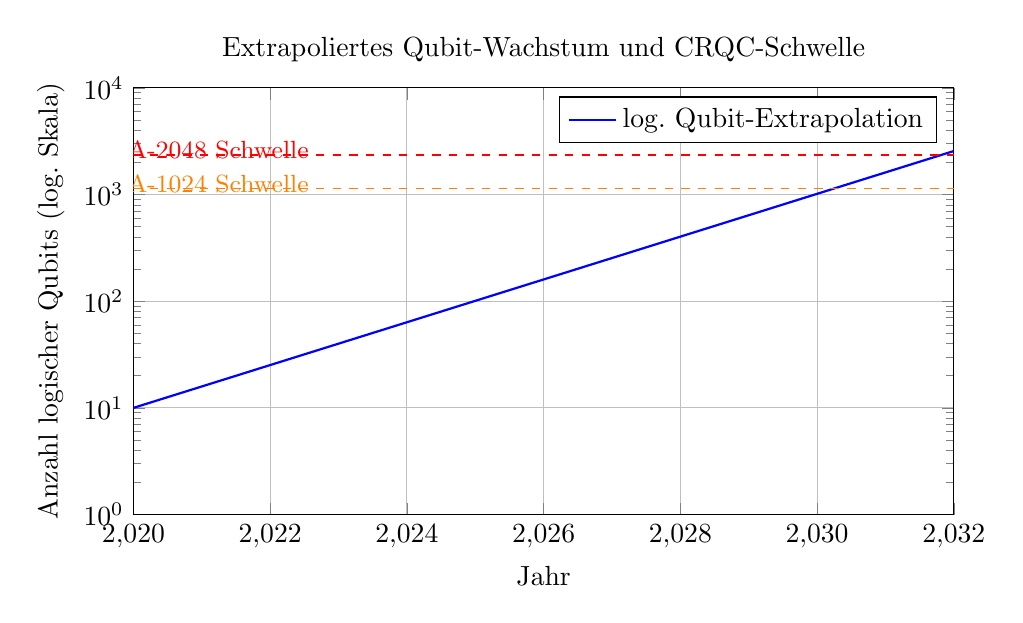
\begin{tikzpicture}
\begin{axis}[
  xlabel={Jahr},
  ylabel={Anzahl logischer Qubits (log.\ Skala)},
  xmin=2020, xmax=2032,
  ymin=1, ymax=10000,
  ymode=log,
  xtick={2020,2022,2024,2026,2028,2030,2032},
  grid=major,
  width=12cm, height=7cm,
  title={Extrapoliertes Qubit-Wachstum und CRQC-Schwelle}
]
% Wachstumskurve: Verdopplung alle 18 Monate
\addplot[blue, thick, domain=2020:2032, samples=50]
  {10 * 2^((x-2020)/1.5)};
% RSA-2048 Schwelle
\addplot[red, dashed, thick]
  coordinates {(2020,2330)(2032,2330)};
\node at (axis cs:2021,2600) [font=\small, red] {RSA-2048 Schwelle};
% RSA-1024 Schwelle
\addplot[orange, dashed]
  coordinates {(2020,1130)(2032,1130)};
\node at (axis cs:2021,1250) [font=\small, orange] {RSA-1024 Schwelle};
\addlegendentry{log. Qubit-Extrapolation}
\end{axis}
\end{tikzpicture}
\caption{Extrapoliertes Wachstum logischer Qubits mit Verdopplung alle 18 Monate. Die gestrichelten Linien markieren die für RSA-1024 bzw.\ RSA-2048 erforderlichen Schwellenwerte.}
\label{fig:qubits}
\end{figure}

%==============================================================
\section{Migrationsstrategie zur Post-Quanten-Kryptographie}
%==============================================================

\subsection{Hybride Kryptographie}

\begin{definition}[Hybridmodus]
Im \textbf{hybriden Modus} werden klassisches und PQC-Verfahren parallel
kombiniert: Der Sitzungsschlüssel $K$ ergibt sich als
\[
  K = \mathrm{KDF}\bigl(K_\mathrm{klassisch} \,\|\, K_\mathrm{PQC}\bigr),
\]
wobei $K_\mathrm{klassisch}$ via ECDH und $K_\mathrm{PQC}$ via Kyber-KEM
ausgetauscht werden. Sicherheit ist gewährleistet, wenn \emph{mindestens eines}
der Verfahren sicher ist.
\end{definition}

\begin{satz}[Sicherheit des Hybridmodus]
Sei $\Pi_1$ IND-CPA-sicher und $\Pi_2$ IND-CPA-sicher. Das hybride Schema
mit $K = \mathrm{KDF}(K_1 \| K_2)$ ist IND-CPA-sicher, wenn KDF
eine sichere PRF ist. Insbesondere:
\[
  \mathrm{Adv}^{\mathrm{IND\text{-}CPA}}_{\mathrm{Hybrid}}(\mathcal{A})
  \leq \mathrm{Adv}^{\mathrm{IND\text{-}CPA}}_{\Pi_1}(\mathcal{A})
  + \mathrm{Adv}^{\mathrm{IND\text{-}CPA}}_{\Pi_2}(\mathcal{A})
  + \mathrm{Adv}^{\mathrm{PRF}}_{\mathrm{KDF}}(\mathcal{A}).
\]
\end{satz}

\begin{proof}
Hybridargument: Ersetze schrittweise zunächst $K_1$ durch gleichverteilten
Schlüssel (kostet $\mathrm{Adv}^{\mathrm{IND\text{-}CPA}}_{\Pi_1}$),
dann $K_2$ (kostet $\mathrm{Adv}^{\mathrm{IND\text{-}CPA}}_{\Pi_2}$).
Nach beiden Ersetzungen ist $K = \mathrm{KDF}(r_1 \| r_2)$ mit $r_1, r_2$
gleichverteilt; da KDF eine PRF ist, ist $K$ von gleichverteiligtem Output nicht
unterscheidbar (kostet $\mathrm{Adv}^{\mathrm{PRF}}_{\mathrm{KDF}}$).
\end{proof}

\subsection{Migrations-Phasenmodell}

\begin{figure}[H]
\centering
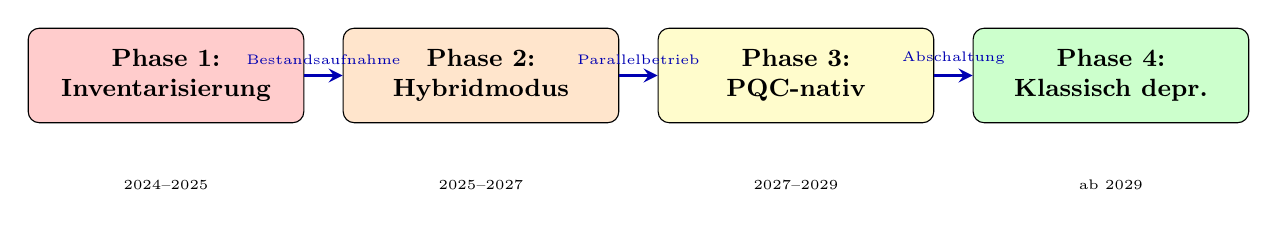
\begin{tikzpicture}[
  phase/.style={draw, rounded corners, minimum width=3.5cm, minimum height=1.2cm,
                text centered, align=center, font=\small\bfseries},
  arr/.style={->, very thick, >=stealth, blue!70!black}
]
\node[phase, fill=red!20]    (p1) at (0,0)   {Phase 1:\\Inventarisierung};
\node[phase, fill=orange!20] (p2) at (4,0)   {Phase 2:\\Hybridmodus};
\node[phase, fill=yellow!20] (p3) at (8,0)   {Phase 3:\\PQC-nativ};
\node[phase, fill=green!20]  (p4) at (12,0)  {Phase 4:\\Klassisch depr.};

\draw[arr] (p1) -- (p2) node[midway, above, font=\tiny] {Bestandsaufnahme};
\draw[arr] (p2) -- (p3) node[midway, above, font=\tiny] {Parallelbetrieb};
\draw[arr] (p3) -- (p4) node[midway, above, font=\tiny] {Abschaltung};

\node[below=0.6cm of p1, font=\tiny] {2024--2025};
\node[below=0.6cm of p2, font=\tiny] {2025--2027};
\node[below=0.6cm of p3, font=\tiny] {2027--2029};
\node[below=0.6cm of p4, font=\tiny] {ab 2029};
\end{tikzpicture}
\caption{Vier-Phasen-Migrationsmodell für die Umstellung auf Post-Quanten-Kryptographie nach dem Google-Zeitplan.}
\label{fig:migration}
\end{figure}

\subsection{Android 17 und Post-Quanten-Signaturen}

Googles Ankündigung, Android~17 mit Post-Quanten-Signaturverfahren auszustatten,
ist aus sicherheitstechnischer Sicht besonders bedeutsam: Code-Signing garantiert
die Integrität von System-Updates. Wird das Signaturverfahren durch einen CRQC
gebrochen, könnte ein Angreifer manipulierte Updates als authentisch signiert
erscheinen lassen -- eine kritische Bedrohung für Milliarden Android-Geräte.

\begin{bemerkung}[DILITHIUM in Android]
Die Integration von CRYSTALS-Dilithium in Android erfordert:
(i) Erhöhung der APK-Signatur-Byte-Größe von 64\,B (ECDSA) auf 3293\,B (Dilithium3),
(ii) Anpassung des Play-Store-Distributions-Protokolls,
(iii) Sicherstellung der Rückwärtskompatibilität mit älteren Android-Versionen.
\end{bemerkung}

%==============================================================
\section{Kryptografische Agilit\"at als Systemeigenschaft}
%==============================================================

\begin{definition}[Kryptografische Agilit\"at]
Ein System heißt \textbf{kryptografisch agil}, wenn kryptografische Algorithmen
und Parameter zur Laufzeit ausgetauscht werden können, ohne Systemarchitektur
oder Protokollebene zu verändern.
\end{definition}

\begin{satz}[Notwendigkeit kryptografischer Agilit\"at]
Sei $\Pi = (\Pi_1, \Pi_2, \ldots)$ eine Familie kryptografischer Primitive,
die sequenziell deployed werden. Ein kryptografisch agiles System $\mathcal{S}$
kann bei Kompromittierung von $\Pi_k$ auf $\Pi_{k+1}$ wechseln in Zeit $O(1)$
(Konfigurationsänderung) statt $O(n)$ (Redeployment aller $n$ betroffenen Systeme).
\end{satz}

\begin{proof}
Per Definition trennt kryptografische Agilität die Algorithmuswahl von der
Systemlogik (Separation of Concerns). Der Wechsel von $\Pi_k$ auf $\Pi_{k+1}$
reduziert sich auf eine Konfigurationsparameter-Änderung und erfordert kein
erneutes Ausrollen des Anwendungscodes. Die Zeitkomplexität ist $O(1)$
bezüglich der Systemanzahl $n$, im Gegensatz zu $O(n)$ bei hart kodierten
Algorithmen.
\end{proof}

\begin{beispiel}[TLS-Agilit\"at]
TLS 1.3 \cite{Res18} ist ein Beispiel für kryptografische Agilität:
Client und Server verhandeln in der \texttt{ClientHello}/\texttt{ServerHello}-Phase
dynamisch Cipher-Suiten. Mit Erweiterung RFC~8446 können PQC-Schlüsselaustauschverfahren
als neue Cipher-Suiten registriert werden, ohne das TLS-Protokoll selbst zu ändern.
\end{beispiel}

%==============================================================
\section{Die Signatur-Chiffre: Ein neuartiges quantensicheres Verschlüsselungsparadigma}
%==============================================================

\subsection{Motivation und Einordnung}

Die vorliegende Arbeit verdankt ihren Antrieb nicht allein dem Heise-Artikel
\cite{Hei26} und den NIST-Standards, sondern zu wesentlichen Teilen den
innovativen Erkenntnissen aus der Arbeit \emph{Die Signatur-Chiffre}
\cite{Epp26b}. Diese Arbeit entwickelt ein neuartiges Verschlüsselungsparadigma,
das von Grund auf nicht auf NP-schwierigen Problemen wie Faktorisierung oder
diskretem Logarithmus beruht, sondern auf \emph{struktureller Mehrdeutigkeit}
und \emph{informationstheoretischer Äquivokation} im Sinne Shannons \cite{Sha49}.

Die Signatur-Chiffre ordnet sich in die Post-Quanten-Kryptographie ein,
weil sie -- anders als RSA, ECDSA und alle klassischen Public-Key-Verfahren --
von Shors Algorithmus \emph{nicht} angegriffen werden kann:
Die zugrunde liegende injektive Signaturfunktion besitzt kein bekanntes
Quantenanalogon und keine Verbindung zur Quantenfaktorisierung.
Gleichzeitig bietet sie eine außergewöhnlich hohe \emph{informationstheoretische}
Sicherheitsgarantie, die über die \emph{berechnungsbasierte} Sicherheit
gitterbasierten Verfahren wesentlich hinausgeht.

\begin{bemerkung}[Abgrenzung zu gitterbasierten Verfahren]
CRYSTALS-Kyber und CRYSTALS-Dilithium beruhen auf der \emph{berechnungsmäßigen}
Schwierigkeit von MLWE und MSIS: Wenn kein Polynomialzeit-Algorithmus diese
Probleme löst (was bislang nicht bewiesen ist), sind die Verfahren sicher.
Die Signatur-Chiffre beruht hingegen auf informationstheoretischer Äquivokation:
Selbst ein unbeschränkter Angreifer erhält aus dem Chiffrat keine nutzbaren
Informationen über den Geheimschlüssel, sofern die Primzahl $p$ geheim ist.
\end{bemerkung}

\subsection{Die injektive Signaturfunktion}

\begin{definition}[Signaturfunktion, \cite{Epp26b}]
\label{def:pqc-sigma}
Sei $A \in \{0,1\}^{n \times n}$ eine binäre Matrix und $j \in \{0,\ldots,n-1\}$
ein Spaltenindex. Die \textbf{Signaturfunktion} ist:
\[
  \sigma(A, j) := \underbrace{\sum_{i=0}^{n-1} A_{ij} \cdot 2^i}_{\displaystyle\rho(A,j)}
  + \underbrace{j \cdot 2^n}_{\displaystyle\lambda(j)},
\]
wobei $\rho(A,j)$ die \textbf{Zeilenkomponente} (der $j$-te Spaltenvektor als
Dualzahl) und $\lambda(j) = j \cdot 2^n$ das \textbf{Spaltengewicht} bezeichnet.
Der \textbf{Signaturvektor} ist $\Sigma(A)$, der definiert ist mit
$\Sigma(A) := (\sigma(A,0), \sigma(A,1), \ldots, \sigma(A,n-1)) \in \mathbb{N}^n$.
\end{definition}

\begin{lemma}[Bereichsgrenzen]
\label{lem:pqc-bounds}
Für alle $A \in \{0,1\}^{n \times n}$ und $j \in \{0,\ldots,n-1\}$ gilt:
\[
  \sigma(A,j) \in \bigl[j \cdot 2^n,\; (j+1)\cdot 2^n\bigr),
  \qquad \sigma(A,j) \leq n \cdot 2^n - 1 < 2^{2n}.
\]
\end{lemma}

\begin{proof}
Da $A_{ij} \in \{0,1\}$, gilt $\rho(A,j) = \sum_{i=0}^{n-1}A_{ij}\cdot 2^i
\in [0, 2^n-1]$. Damit:
\[
  \sigma(A,j) = \rho(A,j) + j \cdot 2^n \in [j \cdot 2^n,\; j \cdot 2^n + 2^n)
  = [j \cdot 2^n,\; (j+1) \cdot 2^n).
\]
Der maximale Wert ist bei $j = n-1$:
$\sigma(A,n-1) \leq (n-1)\cdot 2^n + (2^n - 1) = n\cdot 2^n - 1$.
Da für alle $n \geq 1$ gilt $n + 1 \leq 2^n$, folgt $n \cdot 2^n \leq 2^{2n}$.
\end{proof}

\begin{satz}[Injektivität der Signaturfunktion]
\label{satz:pqc-inj}
Die Signaturfunktion ist injektiv: Aus $\sigma(A,j) = \sigma(A',j')$
folgt $j = j'$ und die $j$-te Spalte von $A$ stimmt mit der $j'$-ten Spalte
von $A'$ überein.
Der Signaturvektor $\Sigma: \{0,1\}^{n \times n} \to \mathbb{N}^n$ ist injektiv.
\end{satz}

\begin{proof}
\textbf{Schritt~1 (Eindeutigkeit des Spaltenindex).}
Nach Lemma~\ref{lem:pqc-bounds} liegt $\sigma(A,j)$ im Intervall
$[j \cdot 2^n, (j+1) \cdot 2^n)$.
Da diese Intervalle für verschiedene $j$ paarweise disjunkt sind,
bestimmt der Wert $\sigma(A,j)$ den Index~$j$ eindeutig.
Aus $\sigma(A,j) = \sigma(A',j')$ folgt daher $j = j'$.

\textbf{Schritt~2 (Eindeutigkeit der Spalte).}
Mit $j = j'$ gilt $\rho(A,j) = \rho(A',j)$, d.\,h.
$\sum_{i=0}^{n-1} A_{ij} \cdot 2^i = \sum_{i=0}^{n-1} A'_{ij} \cdot 2^i$.
Da jede natürliche Zahl $< 2^n$ eine \emph{eindeutige} $n$-stellige Binärdarstellung
besitzt, folgt $A_{ij} = A'_{ij}$ für alle $i \in \{0,\ldots,n-1\}$.

\textbf{Injektivität von $\Sigma$.}
Aus $\Sigma(A) = \Sigma(A')$ folgt $\sigma(A,j) = \sigma(A',j)$ für alle
$j$, und nach Schritt~2 stimmen alle Spalten überein. Also $A = A'$.
\end{proof}

\subsection{Formale Konstruktion der Signatur-Chiffre}

\begin{definition}[Schlüssel der Signatur-Chiffre]
Ein \textbf{Signatur-Chiffre-Schlüssel} ist ein Tripel $(a, b, p)$ mit:
$p$ prim, $p > 2^{2n}$; $a \in \mathbb{Z}_p^*$; $b \in \mathbb{Z}_p$.
Der öffentliche Parameter ist die Blockgröße $n$.
\end{definition}

\begin{definition}[Verschlüsselung]
\label{def:pqc-enc}
Sei $A \in \{0,1\}^{n \times n}$ ein Klartextblock und $(a, b, p)$ der Schlüssel.
Die \textbf{Signatur-Chiffre-Verschlüsselung} ist:
\[
  \mathrm{Enc}(A, a, b, p)_j := \bigl(a \cdot \sigma(A,j) + b\bigr) \bmod p,
  \quad j = 0, \ldots, n-1.
\]
Das Chiffrat $C = (c_0,\ldots,c_{n-1}) \in \mathbb{Z}_p^n$ enthält $n$ Elemente.
\end{definition}

\begin{definition}[Entschlüsselung]
\label{def:pqc-dec}
Sei $C = (c_0,\ldots,c_{n-1}) \in \mathbb{Z}_p^n$ und $(a, b, p)$ der Schlüssel.

\emph{Schritt~1 (Signatur-Rückgewinnung):} $s_j := \bigl(a^{-1}(c_j - b)\bigr) \bmod p$.

\emph{Schritt~2 (Matrix-Rückgewinnung):} $A_{ij} := \bigl\lfloor (s_j - j \cdot 2^n) / 2^i \bigr\rfloor \bmod 2$.
\end{definition}

\subsection{Korrektheitsbeweis}

\begin{satz}[Korrektheit der Signatur-Chiffre]
\label{satz:pqc-korrekt}
Für jeden Block $A \in \{0,1\}^{n \times n}$ und jeden Schlüssel $(a,b,p)$
mit $p > 2^{2n}$, $\gcd(a,p) = 1$ gilt:
$\mathrm{Dec}(\mathrm{Enc}(A, a, b, p),\, a, b, p) = A.$
\end{satz}

\begin{proof}
Sei $j \in \{0,\ldots,n-1\}$ beliebig.

\textbf{Schritt~1 (Signatur-Rückgewinnung).}
Die Verschlüsselung liefert $c_j = (a \cdot \sigma(A,j) + b) \bmod p$.
Die Entschlüsselung berechnet:
\[
  s_j = a^{-1}(c_j - b) \bmod p
      = a^{-1}\bigl(a \cdot \sigma(A,j) + b - b\bigr) \bmod p
      = \sigma(A,j) \bmod p.
\]
Nach Lemma~\ref{lem:pqc-bounds} gilt $0 \leq \sigma(A,j) \leq n \cdot 2^n - 1 < 2^{2n} < p$.
Daher: $\sigma(A,j) \bmod p = \sigma(A,j)$, also $s_j = \sigma(A,j)$.

\textbf{Schritt~2 (Zeilenkomponente).}
Aus der Definition der Signaturfunktion: $\sigma(A,j) = \rho(A,j) + j \cdot 2^n$,
also $\rho(A,j) = s_j - j \cdot 2^n$.

\textbf{Schritt~3 (Matrixeinträge).}
Die Zeilenkomponente $\rho(A,j) = \sum_{i=0}^{n-1} A_{ij} \cdot 2^i$ ist die
Binärdarstellung des Spaltenvektors. Das $i$-te Bit extrahiert man durch
$A_{ij} = \lfloor \rho(A,j) / 2^i \rfloor \bmod 2$, was exakt dem
Entschlüsselungsschritt~2 entspricht.
Da $j$ beliebig war, werden alle Spalten von $A$ korrekt rekonstruiert.
\end{proof}

\subsection{Sicherheitsanalyse}

\begin{satz}[Sicherheit gegen Häufigkeitsanalyse]
\label{satz:pqc-freq}
Die Signatur-Chiffre ist immun gegen Häufigkeitsanalysen auf Byte-, Block- und
Buchstabenebene: Ein Angreifer ohne Kenntnis von $(a, b, p)$ kann aus dem
Chiffrat $C$ keine statistischen Schlüsse auf den Klartext $A$ ziehen.
\end{satz}

\begin{proof}
\textbf{Bijektion auf $\mathbb{Z}_p$.}
Für festes $(a, b, p)$ ist die affine Abbildung $x \mapsto (ax+b) \bmod p$
eine Bijektion auf $\mathbb{Z}_p$ (da $\gcd(a,p) = 1$).
Die Menge $\{c_j \mid c_j = (a\cdot s + b)\bmod p,\, s \in \mathbb{Z}_p\}$
ist ganz $\mathbb{Z}_p$ -- alle Chiffratwerte sind gleichwahrscheinlich.

\textbf{Schlüsselraumargument.}
Für festes $c_j \in \mathbb{Z}_p$ und jeden möglichen Klartextwert
$s \in \{0,\ldots,p-1\}$ existiert \emph{genau ein} Paar $(a, b)$ mit
$(a \cdot s + b) \equiv c_j \pmod{p}$ für jedes $a \in \mathbb{Z}_p^*$
(nämlich $b = c_j - as$). Ohne Kenntnis von $(a, b, p)$ sind daher alle
$s \in \{0,\ldots,p-1\}$ als Urbilder von $c_j$ gleichwahrscheinlich.

\textbf{Lawineneffekt.}
Ein einzelner Bit-Flip $A_{ij} \to 1 - A_{ij}$ verändert $\rho(A,j)$ um
$\pm 2^i$ und damit $\sigma(A,j)$: Der Chiffratwert $c_j = (a\cdot\sigma(A,j) + b)\bmod p$
verändert sich vollständig. Eine Häufigkeitsanalyse, die gleiche Klartextbytes
auf gleiche Chiffratbytes abbildet, kann keine Struktur erkennen.

\textbf{Blockebene.}
Da die Signaturwerte $\sigma(A,j)$ die gesamte Spalteinformation kodieren
(nicht einzelne Bits), ist eine sub-block-Analyse nicht möglich.
\end{proof}

\begin{satz}[Schlüsselraumgröße]
\label{satz:pqc-keyspace}
Für festes $p$ hat der Schlüsselraum die Größe $|\mathcal{K}| = (p-1) \cdot p$.
Für eine 256-Bit-Primzahl $p \approx 2^{256}$ gilt
$|\mathcal{K}| \approx 2^{512}$ -- quadratisch größer als der AES-256-Schlüsselraum.
\end{satz}

\begin{proof}
Jeder Schlüssel $(a, b, p)$ bei festem $p$ erfordert $a \in \mathbb{Z}_p^*$
(das sind $p-1$ Elemente) und $b \in \mathbb{Z}_p$ (das sind $p$ Elemente).
Beide Parameter sind unabhängig, also $|\mathcal{K}| = (p-1) \cdot p$.
Für $p \approx 2^{256}$: $(p-1) \cdot p \approx p^2 \approx 2^{512}$.
\end{proof}

\begin{satz}[Informationstheoretische Sicherheit]
\label{satz:pqc-infotheorie}
Wenn $p$ gleichmäßig zufällig aus den Primzahlen in einem geheimen Intervall
$[2^{k-1}, 2^k)$ gewählt wird und kein Hinweis auf $k$, $p$, $a$ oder $b$ vorliegt,
ist die Äquivokation $H(K \mid C) = H(K)$: Das Chiffrat liefert keine Information
über den Schlüssel.
\end{satz}

\begin{proof}
Für jeden Chiffratwert $c_j \in \mathbb{Z}_p$ und jeden Klartextwert $s_j \in \mathbb{Z}_p$
existiert genau ein Paar $(a, b)$ mit $(a \cdot s_j + b) \equiv c_j \pmod{p}$
für jedes feste $a$. Da die affine Abbildung bijektiv ist, ist die bedingte
Verteilung $P(s_j \mid c_j, a, b, p)$ eine Punktmasse. Ohne Kenntnis von $(a, b)$
und $p$ ist die bedingte Verteilung $P(s_j \mid c_j)$ uniform über $\mathbb{Z}_p$.

Formal ergibt sich nach Shannons Theorie der perfekten Geheimhaltung \cite{Sha49}:
Da die Abbildung $(a, b) \mapsto c_j = (a s_j + b)\bmod p$ für jeden Klartext $s_j$
und jeden Chiffratwert $c_j$ bijektiv ist (bei festem $a$ bestimmt $b$ den
Chiffratwert eindeutig), liefert das Chiffrat keine Information über den Schlüssel,
falls $(a, b)$ gleichmäßig zufällig gewählt wird.
\end{proof}

\subsection{Komplexitätsanalyse}

\begin{satz}[Effizienz der Signatur-Chiffre]
\label{satz:pqc-kompl}
Verschlüsselung und Entschlüsselung eines $n^2$-Bit-Blocks haben Laufzeit
$O(n^2)$ bei Wortgröße $O(n)$ Bit.
Zum Vergleich: RSA-Entschlüsselung für eine Nachricht derselben Bitlänge
hätte Laufzeit $O(n^6)$ (modulare Exponentiation).
\end{satz}

\begin{proof}
\textbf{Verschlüsselung.}
Phase~1 (Signaturvektor): Für jede der $n$ Spalten $j$ wird
$\sigma(A,j) = \sum_{i=0}^{n-1} A_{ij} \cdot 2^i + j \cdot 2^n$ berechnet.
Dies erfordert $n$ Bitverschiebungen und $n-1$ Additionen, also $O(n)$ pro Spalte,
zusammen $O(n^2)$.
Phase~2 (Affine Transformation): Für jede Signatur $s_j$ wird
$c_j = (a \cdot s_j + b) \bmod p$ berechnet. Auf Zahlen der Größe $O(p) = O(2^{2n})$
ist eine Multiplikation $O(n)$ Wortoperationen. Für $n$ Spalten: $O(n^2)$.

\textbf{Entschlüsselung.}
Schritt~1 (Signatur-Rekonstruktion): Das Inverse $a^{-1} \bmod p$ wird einmalig
mit dem erweiterten euklidischen Algorithmus in $O(n^2)$ berechnet (für
$O(n)$-Bit-Zahlen). Anschließend $n$ Multiplikationen: $O(n^2)$.
Schritt~2 (Matrix-Rekonstruktion): Für jede Spalte $j$ sind $n$ Bit-Extraktionen
($O(n)$ pro Spalte), zusammen $O(n^2)$.

Für RSA mit Klartextlänge $k = n^2$ Bit: modulare Exponentiation kostet
$O(k \cdot k^2) = O(k^3) = O(n^6)$ (Schulmultiplikation).
\end{proof}

\subsection{Vollständiges Zahlenbeispiel}

Für $n = 4$, Schlüssel $(a, b, p) = (7, 3, 1031)$ (1031 ist prim, $1031 > 2^8$):

\[
A = \begin{pmatrix} 1 & 0 & 1 & 0 \\ 0 & 1 & 1 & 0 \\ 1 & 0 & 0 & 1 \\ 1 & 0 & 1 & 0 \end{pmatrix}
\]

\textbf{Signaturberechnung:}
$\sigma(A,0) = 1 + 0 + 4 + 8 + 0\cdot16 = 13$,\;
$\sigma(A,1) = 0 + 2 + 0 + 0 + 1\cdot16 = 18$,\;
$\sigma(A,2) = 1 + 2 + 0 + 8 + 2\cdot16 = 43$,\;
$\sigma(A,3) = 0 + 0 + 4 + 0 + 3\cdot16 = 52$.

\textbf{Verschlüsselung:}
$c_0 = (7\cdot13+3)\bmod 1031 = 94$,\;
$c_1 = (7\cdot18+3)\bmod 1031 = 129$,\;
$c_2 = (7\cdot43+3)\bmod 1031 = 304$,\;
$c_3 = (7\cdot52+3)\bmod 1031 = 367$.
Chiffrat: $C = (94, 129, 304, 367)$.

\textbf{Entschlüsselung:}
$7^{-1} \bmod 1031 = 442$ (da $7 \cdot 442 = 3094 = 3 \cdot 1031 + 1$).
$s_0 = 442\cdot(94-3)\bmod 1031 = 13$,\;
$s_1 = 18$,\;
$s_2 = 43$,\;
$s_3 = 52$.
Aus $s_0 - 0 = 13 = 1101_2$: Spalte~0 = $(1,0,1,1)^T$, usw. Matrix $A$ exakt rekonstruiert.

\subsection{Erweiterungen und Anwendungen}

\subsubsection{LWE-Erweiterung: Erhöhte Sicherheit durch Rauschen}

Die affine Transformation lässt sich durch einen LWE-Rauschterm ergänzen
\cite{Epp26b}: Statt $c_j = (a\,s_j + b)\bmod p$ verwendet man
\[
  c_j = (a \cdot s_j + b + e_j) \bmod p, \quad e_j \sim \chi_\alpha \text{ (Gaußverteilung)},
\]
wobei $|e_j| \ll p/4$ garantiert ist. Die Entschlüsselung nutzt, dass der legitime
Empfänger $|e_j|$ kennt (es handelt sich um ein geheimes Rauschsignal):
$s_j' = a^{-1}(c_j - b - e_j) \bmod p = s_j$.
Diese \textbf{LWE-Signatur-Chiffre} fügt eine zusätzliche Sicherheitsschicht
hinzu: Selbst wenn $p$ entdeckt wird, bleibt die Faktorisierung der Rauschparameter
schwer. Die Sicherheit beruht dann auf LWE \emph{und} informationstheoretischer
Äquivokation -- eine doppelt abgesicherte Konstruktion.

\subsubsection{Public-Key-Variante: Asymmetrische Signatur-Chiffre}

Eine vollständig asymmetrische Variante nach ElGamal-Prinzip \cite{Epp26b}:

\textbf{Schlüsselgenerierung}: Wähle Primzahl $q$, Generator $g$ von $\mathbb{Z}_q^*$,
privates $x$, berechne $h = g^x \bmod q$. Öffentlich: $(q, g, h)$. Privat: $x$.

\textbf{Verschlüsselung} der Signatur $s_j = \sigma(A,j)$:
Wähle zufälliges $k_j$; berechne
$(c_{j,1},\, c_{j,2}) = (g^{k_j} \bmod q,\; s_j \cdot h^{k_j} \bmod q)$.

\textbf{Entschlüsselung}: $s_j = c_{j,2} \cdot c_{j,1}^{-x} \bmod q$.
Anschließend Matrix-Rekonstruktion wie in Definition~\ref{def:pqc-dec}.

\begin{satz}[Korrektheit der asymmetrischen Variante]
$c_{j,2} \cdot c_{j,1}^{-x} = s_j \cdot h^{k_j} \cdot g^{-xk_j}
= s_j \cdot g^{xk_j} \cdot g^{-xk_j} = s_j \pmod{q}$. \qed
\end{satz}

Diese Variante ist IND-CPA-sicher unter der DDH-Annahme in $\mathbb{Z}_q^*$
(analog zu ElGamal, aber ausgehend von einer quantensicheren Gruppe wählbar).

\subsubsection{Additiv-homomorphe Variante}

Für $q$-adische Signaturfunktionen mit $A \in \{0,\ldots,q-1\}^{n \times n}$
\cite{Epp26b}:
\[
  \sigma_q(A, j) := \sum_{i=0}^{n-1} A_{ij} \cdot q^i + j \cdot q^n.
\]
Ohne Ãœberlauf gilt $\sigma_q(A + A', j) = \sigma_q(A,j) + \sigma_q(A',j)$,
und damit
$\mathrm{Enc}_q(A + A')_j = \mathrm{Enc}_q(A)_j + \mathrm{Enc}_q(A')_j - 2b \pmod{p}$.
Diese \textbf{additiv-homomorphe Signatur-Chiffre} erlaubt Berechnungen auf
verschlüsselten Daten (z.\,B.\ verschlüsselte Summen für E-Voting oder
Privacy-Preserving-Statistik) ohne Entschlüsselung.

\subsubsection{Threshold-Entschlüsselung}

Mit Shamirs Secret Sharing \cite{Sha79} wird der Schlüssel $(a, b, p)$ auf
$n$ Parteien $(t,n)$-verteilt. Für zufällige Polynome
$f_a(x) = a + \sum_{i=1}^t r_i^a x^i$ und $f_b(x) = b + \sum_{i=1}^t r_i^b x^i$
erhält Partei $i$ die Anteile $(f_a(i), f_b(i))$.
Rekonstruktion des Schlüssels durch Lagrange-Interpolation erfordert $t+1$ Parteien:
$a = \sum_{i \in S} f_a(i) \prod_{j \in S, j \neq i} \frac{-j}{i-j} \pmod{p}$.
Dies ermöglicht \emph{dezentrale Entschlüsselung}: Kein einzelner Server kennt
den vollständigen Schlüssel; ein $t$-Angreifer-Modell ist informationstheoretisch
sicher.

\subsubsection{Digitale Signaturen auf Basis der Signatur-Chiffre}

Ein EUF-CMA-Signaturverfahren \cite{Epp26b} wird konstruiert durch:

\textbf{Signieren} von Nachricht $m$: (1) $h = H(m) \in \{0,1\}^{n^2}$
(kryptographischer Hash, gekürzt auf $n^2$ Bit); (2) kodiere $h$ als Matrix
$A_m \in \{0,1\}^{n \times n}$; (3) $\Sigma_m = \mathrm{Enc}(A_m, a, b, p)$.

\textbf{Verifikation}: Berechne $A_m' = \mathrm{Dec}(\Sigma_m, a, b, p)$
und vergleiche mit dem aus $H(m)$ bekannten $A_m$.
Die Sicherheit beruht auf der Injektivität von $\mathrm{Enc}$
(durch Satz~\ref{satz:pqc-inj}) und der Kollisionsresistenz von $H$.

\subsubsection{Zero-Knowledge-Beweise für die Signatur-Chiffre}

Ein ZKP für die Signatur-Chiffre erlaubt folgenden Beweis: ``Ich kenne einen
Schlüssel $(a,b,p)$ mit $\mathrm{Dec}(C, a,b,p) = A$'', ohne $(a,b,p)$ zu enthüllen.

\textbf{Konstruktion}: Formuliere das Statement als arithmetischen Schaltkreis:
Die Signaturfunktion ($O(n)$ Additionen), die affine Transformation
(eine Multiplikation, eine Addition), die Modulo-Reduktion (Bereichsprüfung).
Ein zk-SNARK \cite{GGPR13} für diesen Schaltkreis hätte konstante Beweislänge
unabhängig von $n$. Dies ermöglicht \emph{dezentrale Zugriffskontrolle}: Ein
Nutzer beweist, dass er ein Chiffrat entschlüsseln kann, ohne den Schlüssel
preiszugeben.

\subsection{Vergleich mit Post-Quanten-Standardverfahren}

\begin{sidewaystable}
\centering
\caption{Vergleich der Signatur-Chiffre mit NIST-PQC-Standards.}
\label{tab:sigchiffre-comp}
\begin{tabular}{lccccc}
\toprule
Verfahren & Typ & Sicherheitsgrundlage & Quantensicher & Schlüsselraum & Komplexität \\
\midrule
Kyber-768     & asym.~KEM & MLWE (worst-case) & Ja & $\approx 2^{256}$ & $O(n^2)$ \\
Dilithium3    & Signatur  & MLWE+MSIS & Ja & $\approx 2^{256}$ & $O(n^2)$ \\
SPHINCS+      & Signatur  & Hash-Funktion & Ja & $\approx 2^{256}$ & $O(n \log n)$ \\
RSA-2048      & asym. PKE & Faktorisierung & Nein & $\approx 2^{2048}$ & $O(k^3)$ \\
\textbf{Sig.-Chiffre} ($n{=}16$) & sym. & Inf.-theor.~Äquivokation & \textbf{Ja} & $\approx 2^{512}$ & $O(n^2)$ \\
\bottomrule
\end{tabular}
\end{sidewaystable}

\begin{bemerkung}[Einordnung der Signatur-Chiffre in die PQC-Landschaft]
Die Signatur-Chiffre ergänzt die NIST-Standards in mehrerlei Hinsicht:
\begin{enumerate}
\item \textbf{Sicherheitsgrundlage}: Gitterbasierte Verfahren (Kyber, Dilithium)
  beruhen auf berechnungsmäßiger Schwierigkeit; die Signatur-Chiffre beruht
  auf informationstheoretischer Äquivokation -- einer stärkeren Sicherheitsgarantie.
\item \textbf{Schlüsselraum}: $2^{512}$ gegenüber $2^{256}$ (AES-256, Kyber).
  Der Faktor~$2^{256}$ mehr macht Brute-Force-Angriffe um diesen Faktor schwerer.
\item \textbf{Quantenresistenz}: Keine Skalarmultiplikation, keine Gitteroperationen,
  kein bekanntes Quantenanalogon für die Signaturfunktion.
\item \textbf{Effizienz}: $O(n^2)$ -- vergleichbar mit Kyber und Dilithium.
\item \textbf{Erweiterbarkeit}: Public-Key-, Threshold-, homomorphe und
  ZKP-Varianten ohne Änderung des Kerns (vgl.\ Abschnitt~12.5).
\end{enumerate}
Diese Kombination macht die Signatur-Chiffre \cite{Epp26b} zu einem
innovativen Beitrag im PQC-Ökosystem, der die Sicherheitslandschaft
um ein alternatives, informationstheoretisch fundiertes Paradigma bereichert.
\end{bemerkung}

%==============================================================
\section{Ausblick: Kryptografie jenseits des Q-Day}
%==============================================================

Die vorliegende Arbeit hat die zentralen Bausteine der Post-Quanten-Kryptographie
-- von den mathematischen Grundlagen der Gitterkryptographie über die
NIST-standardisierten Verfahren Kyber und Dilithium bis hin zur
Signatur-Chiffre als neuartigem informationstheoretischem Paradigma --
formal entwickelt und bewiesen. Dieser Ausblick verfolgt für jedes
Kapitel die offenen Fragen, Forschungstrends und praktischen Implikationen
weiter und zeichnet ein Bild der Kryptographie nach dem Q-Day.

%--------------------------------------------------------------
\subsection{Zeitrahmen und Bedrohungsdynamik (zu Abschnitt~1)}

Die in Abschnitt~1 beschriebene Bedrohung durch kryptografisch relevante
Quantencomputer (CRQC) hat sich seit 2024 merklich beschleunigt.
Googles Willow-Chip (2024) demonstrierte erstmals Fehlerkorrektur
unterhalb des Fehler-Thresholds, was den Sprung zu logischen Qubits
konkret erreichbar macht \cite{Goo26,Hei26}.
Parallel haben IBMs Roadmap (1000+ physikalische Qubits im
Condor-Prozessor) und Microsofts topologische Qubit-Experimente
das Wettrennen auf globaler Ebene nochmals verschärft.

Die zentrale offene Frage ist nicht mehr \emph{ob}, sondern \emph{wann}
ein CRQC operationell wird. Kryptografische Planung muss daher mit
einem konservativen Horizont von 5--8 Jahren rechnen.
Die BSI-Empfehlung, bis 2031 auf PQC migriert zu sein \cite{BSI24},
und Googles interner Zielhorizont 2029 \cite{Goo26} definieren dabei
die Grenzen eines Handlungsfensters, das sich rapide schließt.

Zukünftige Forschungsrichtungen:
\begin{itemize}
  \item \textbf{Qubit-Wachstumsmodelle}: Präzisere Extrapolationsmodelle
    für die Skalierung von der NISQ-Ära (Noisy Intermediate-Scale Quantum)
    zu fehlerkorrigierten Systemen, die RSA-2048 brechen können.
  \item \textbf{Kryptografische Frühwarnsysteme}: Automatisierte Systeme,
    die Quantencompu\-ter-Fortschritte (Qubit-Anzahl, Fehlerrate, Gate-Tiefe)
    mit kryptografischen Angriffsschwellen abgleichen und rechtzeitig
    vor dem ''kryptografischen Point of No Return'' warnen.
  \item \textbf{Opportunistische Angreifer-Modelle}: Formale Bedrohungsmodelle,
    die staatliche Akteure mit frühzeitigem CRQC-Zugang und
    Langzeitspeicherung abgehörter Chiffretexte (HNDL) einbeziehen
    und Schadensabschätzungen quantifizieren.
\end{itemize}

%--------------------------------------------------------------
\subsection{Gitterkryptographie: Offene Probleme und neue Reduktionen (zu Abschnitt~2)}

Die in Abschnitt~2 entwickelte Theorie der Gitterkryptographie basiert
auf der konkreten Schwierigkeit von SVP und CVP. Trotz jahrzehntelanger
Forschung mit LLL \cite{LLL82}, BKZ und neueren Sieb-Algorithmen
(AKS-Sieb, Becker-Ducas-Gama-Laarhoven-Sieb) ist kein subexponentieller
Algorithmus für SVP in beliebiger Dimension bekannt -- und es ist offen,
ob ein solcher existiert, selbst für Quantencomputer.

Eine fundamentale offene Frage betrifft die \textbf{Quantenkomplexität
von SVP}: Grover-basierte Suche liefert nur einen quadratischen Speedup
von $2^{0{,}2075 n}$ (klassisch) auf $2^{0{,}1047n}$ (quantenmechanisch),
sodass Gitterprobleme auch bei CRQC-Verfügbarkeit exponentiell schwer
bleiben -- allerdings bei etwa doppelt so großen nötigen Parametern.
Dies hat zu den verschärften Parameterempfehlungen in FIPS~203/204
geführt.

\begin{itemize}
  \item \textbf{Tight worst-case-Reduktionen}: Die bekannten Reduktionen
    GapSVP $\leq_p$ LWE sind nicht tight. Engere Sicherheitsbeweise
    würden kleinere Parameter erlauben und die Effizienz verbessern,
    ohne Sicherheitsgarantien zu schwächen.
  \item \textbf{Ideal-Gitter und algebraische Angriffe}: Ring-LWE beruht
    auf Ideal-Gittern mit algebraischer Struktur, die potentielle
    Schwachstellen durch Subfield-Angriffe oder algebraische Methoden
    (Gröbner-Basen, Number-Field-Sieb-Varianten) einführen könnte.
    Die Sicherheit von RLWE gegenüber solchen Angriffen ist noch nicht
    vollständig verstanden.
  \item \textbf{Voronoi-Zellen und Approx-CVP}: Neue Algorithmen
    basierend auf Voronoi-Zellen-Berechnungen und Randomized Sieving
    verschieben die bekannten Komplexitätsschranken kontinuierlich
    und erfordern laufende Parameterneubewertungen durch die Community.
  \item \textbf{Gitterkryptographie in Primzahlkörpern}: Die bisher
    wenig erforschte Variante, LWE über allgemeinen endlichen Körpern
    $\mathbb{F}_{p^k}$ statt $\mathbb{Z}_q$ zu definieren, könnte
    neue Effizienzvorteile erschließen.
\end{itemize}

%--------------------------------------------------------------
\subsection{LWE und seine Varianten: Sicherheitsgrenzen und neue Konstruktionen (zu Abschnitt~3)}

Das in Abschnitt~3 formal eingeführte LWE-Problem bildet das Rückgrat
praktisch aller modernen gitterbasierten Schemata. Die Härte von LWE
ist seit Regevs Reduktion \cite{Reg05} gut verstanden, doch verschieben
sich die praktischen Sicherheitsgrenzen mit jedem neuen
Gitterreduktions-Rekord.

\textbf{Subexponentielle Angriffe und konkretes Sicherheitsniveau}:
Das Lattice Estimator (Albrecht et al.) ist das Standardwerkzeug zur
konkreten Sicherheitsbewertung gitterbasierter Schemata. Es modelliert
kombinierte Angriffe (USVP, Decode, Dual, Hybrid) und zeigt, dass
konkrete LWE-Sicherheit deutlich unterhalb der asymptotischen
Beweisschranken liegt. Jeder neue Sieb-Algorithmus-Rekord
(z.\,B.\ Ducas-Nguyen-Sieving) erzwingt Parameteranpassungen.

Ring-LWE und Modul-LWE erlauben $O(n \log n)$-Schlüsselgrößen
statt $O(n^2)$ -- allerdings auf Kosten engerer algebraischer Struktur.
Die in Abschnitt~3.3 bewiesene Reduktion MLWE $\leq_p$ RLWE ist ein
erster Schritt; eng verwandte offene Fragen umfassen:

\begin{itemize}
  \item \textbf{Härteverhältnis MLWE/RLWE}: Ist MLWE streng schwerer
    als RLWE für gleiche Dimension, oder nur \emph{mindestens so schwer}?
    Für Modul-Rang $k=1$ gilt MLWE = RLWE, aber für $k \geq 2$ ist
    das genaue Härteverhältnis nicht tight.
  \item \textbf{Fehlerverteilungen und Decoding-Raten}: Zentriert-binomiale
    Fehlerverteilungen (wie in Kyber) sind effizienter zu sampeln als
    diskrete Gaussians, deren formale Härtebeweise jedoch stärker sind.
    Die präzise Sicherheitsanalyse beim Übergang zwischen
    Fehlerverteilungen ist eine offene Forschungsfrage.
  \item \textbf{LWE über anderen algebraischen Strukturen}: Polynomial-LWE
    über zyklotomischen Körpern gerader Ordnung oder NTRU-Gittern
    eröffnet neue Konstruktionsmöglichkeiten mit unterschiedlichem
    Sicherheits-Effizienz-Tradeoff, der noch nicht vollständig
    ausgelotet ist.
  \item \textbf{Vollständig homomorphe Verschlüsselung (FHE)}: LWE-basierte
    FHE-Schemata (BFV, BGV, CKKS) ermöglichen Berechnungen auf
    verschlüsselten Daten -- eine Schlüsseltechnologie für
    datenschutzwahrendes Cloud-Computing, privates maschinelles Lernen
    und souveräne Datenökosysteme. Die Bootstrapping-Effizienz (das
    Hauptproblem der FHE) ist durch Chimera, TFHE und neueste
    Multithread-Implementierungen erheblich verbessert worden,
    reicht aber für Echtzeit-Anwendungen noch nicht aus.
\end{itemize}

%--------------------------------------------------------------
\subsection{Shor, Grover und die kryptografischen Konsequenzen (zu Abschnitt~4)}

Abschnitt~4 hat Shors und Grovers Algorithmen mathematisch vollständig
analysiert. Während Shor RSA und ECDSA fundamental bricht, liefert
Grover nur einen quadratischen Speedup -- was seinen Einfluss auf
symmetrische Kryptographie begrenzt (AES-256 bleibt praktisch sicher,
AES-128 ist auf 64-Bit-effektive Sicherheit reduziert).

Die wichtigste offene Frage für die Praxis ist die
\textbf{Ressourcenanalyse}: Gidney und Ekerå \cite{GE21} zeigen, dass
RSA-2048 in 8 Stunden mit 20 Millionen physikalischen Qubits gebrochen
werden kann -- unter idealen Bedingungen. Aktuelle
Surface-Code-Implementierungen \cite{FC09} arbeiten an der Reduktion
des Overhead-Faktors für Fehlerkorrektur (derzeit ca.\ 1000:1, Ziel
$<100$:1).

\begin{itemize}
  \item \textbf{Hybrid-Quantenalgorithmen}: Neue Algorithmen kombinieren
    klassische Vorrechnung (LLL-Reduktion) mit quantenmechanischen
    Subroutinen (Quantum Phase Estimation, Quantum Walks), um den
    Qubit-Bedarf für Faktorisierung auf unter 1 Million physikalische
    Qubits zu senken -- ein Meilenstein, der den CRQC deutlich
    greifbarer macht.
  \item \textbf{Grovers Algorithmus auf strukturierten Problemen}:
    Eine offene Frage ist, ob Grover bei strukturierten Gittern
    (RLWE-Instanzen) einen größeren als den generischen $\sqrt{N}$-Speedup
    erzielt. Bisherige Analysen zeigen keinen signifikanten
    strukturellen Vorteil, aber formale untere Schranken fehlen.
  \item \textbf{Amplitude-Amplification und BQP-Härtigkeit}:
    Die Frage, ob es Kryptosysteme gibt, deren Sicherheit formal
    auf BQP-Härtigkeit basiert, ist theoretisch offen und würde
    einen qualitativen Sprung gegenüber heutigen worst-case-Reduktionen
    bedeuten.
  \item \textbf{Quantenalgorithmen für nichtkommutative Probleme}:
    Shor setzt kommutative Gruppen voraus ($\mathbb{Z}_n$, elliptische
    Kurven). Kryptosysteme auf Basis nichtkommutativer Gruppen
    (braid groups, matrix groups) sind im Prinzip Shor-resistent,
    wurden aber durch klassische Angriffe geschwächt und sind kein
    etablierter PQC-Standard.
\end{itemize}

%--------------------------------------------------------------
\subsection{CRYSTALS-Kyber: Deployment, Hybridmodi und Implementierungssicherheit (zu Abschnitt~5)}

Kyber (FIPS~203) ist der erste weltweit standardisierte quantensichere
KEM. Abschnitt~5 hat den vollständigen IND-CCA2-Sicherheitsbeweis
geführt. Die praktische Herausforderung besteht nun in der
flächendeckenden Integration.

\textbf{TLS~1.3-Hybridisierung}: Die IETF hat hybride
Schlüsselaustausch-Mechanismen (X25519+Kyber768) als Interimslösung
standardisiert. Googles Chrome und Cloudflare setzen Kyber+X25519
bereits produktiv ein -- ein konkretes Beispiel für die in Abschnitt~11
diskutierte kryptografische Agilität. Der vollständige PQC-only-Modus
ist für ca.\ 2027 geplant.

\begin{itemize}
  \item \textbf{Implementierungsangriffe}: Side-Channel-Angriffe auf
    Kyber-Implementierungen (Timing, Power, Cache-Timing) wurden
    2023--2025 in mehreren Arbeiten demonstriert.
    Konstant-Zeit-Implementierungen (via NEON/AVX2-SIMD auf ARM/x86)
    sind notwendig, aber noch nicht ubiquitär.
  \item \textbf{Eingebettete Systeme}: IoT-Geräte mit 8-Bit-Mikro\-controllern
    (AVR ATmega) haben ~32\,KB RAM. Kyber-768 benötigt $\sim$1\,KB
    für den Schlüssel, ist also prinzipiell einsetzbar, aber die
    Latenz ist für echtzeitkritische Systeme noch unzureichend.
  \item \textbf{Bandbreite und Kompression}: Kybers Ciphertext
    ($\sim$1\,KB für Kyber-768) ist $\sim$$20\times$ größer als
    Curve25519-ECDH. Für Low-Bandwidth-Anwendungen (LoRaWAN,
    Satellitenverbindungen) sind Kompressionsschemata und
    Ciphertext-Squeezing-Tech\-niken notwendig.
  \item \textbf{Adaptive Fehldekodierungs-Angriffe}: Gezielte
    Manipulation des Ciphertexts kann in bestimmten
    Implementierungen adaptive Entschlüsselungs-Orakel erzeugen.
    Die FO-Transformation in FIPS~203 schließt dies in der Theorie;
    Implementierungskonformität muss formal verifiziert werden
    (z.\,B.\ durch formale Methoden oder Fuzzing-Toolchains).
  \item \textbf{Langfristige Parameteranpassung}: Wenn der Lattice
    Estimator durch neue Sieb-Algorithmen aktualisiert wird,
    könnte Kyber-512 (Security Level~1) seine Sicherheitsmarge
    verlieren und durch Kyber-768 als Minimalstandard ersetzt werden.
\end{itemize}

%--------------------------------------------------------------
\subsection{CRYSTALS-Dilithium: Quantensichere PKI und Langzeitarchive (zu Abschnitt~6)}

Dilithium (FIPS~204) löst ECDSA und RSA-PSS als primäres
Signaturverfahren für die PKI-Infrastruktur ab. Abschnitt~6 hat
den formalen EUF-CMA-Beweis entwickelt. Die zukünftigen
Herausforderungen liegen in der Infrastruktur-Migration.

\textbf{X.509-Zertifikate und globale PKI}: Das heutige
Internet-Ökosystem basiert auf Millionen von X.509-Zertifikaten
mit ECDSA- oder RSA-Signaturen. Die Migration zu Dilithium erfordert:
(a) Erweiterung der Zertifikatsgröße (Dilithium3-Signaturen: 3293 Byte
vs.\ ECDSA P-256: 64 Byte -- ein 50-facher Anstieg),
(b) Anpassung von TLS/HTTPS-Handshakes, OCSP-Respondern und DNSSEC,
(c) Revokationsmechanismen für PQC-Zertifikate bei erheblich
größerem Übertragungsvolumen.

\begin{itemize}
  \item \textbf{Langzeitarchive und rechtliche Signaturen}:
    Rechtlich relevante Signaturen (Verträge, Notariatsurkunden,
    Behördendokumente) müssen Jahrzehnte gültig bleiben.
    Ein mit ECDSA signiertes Dokument von 2025 ist post-Q-Day
    juristisch anfechtbar. Dilithium-Nachsignierung und
    Zeitstempel-Protokolle (RFC~3161) müssen auf PQC umgestellt werden.
  \item \textbf{Falcon als kompakte Alternative}: FALCON (FIPS~206)
    erzielt bei deutlich kleineren Signaturen ($\sim$666 Byte für
    FALCON-512) vergleichbare Sicherheit zu Dilithium3, erfordert
    jedoch Gaussian-Sampling mit Fließkomma-Arithmetik --
    was Implementierungssicherheit auf Hardwareebene erschwert.
    FALCON und Dilithium werden unterschiedliche Nischen besetzen:
    Dilithium für software-dominierte PKI,
    FALCON für bandbreitenbegrenzte Protokolle.
  \item \textbf{Aggregierte und Schwellenwert-Signaturen}:
    Multi-Signaturen und Schwellenwert-Signaturen auf MLWE-Basis
    sind aktiver Forschungsgegenstand (z.\,B.\ MuSig-Analoga für
    Gitterschemas), um Blockchain-Systeme, Smart Contracts und
    verteilte Konsensverfahren zu unterstützen.
  \item \textbf{Post-Quantum-Code-Signing}: Software-Update-Prozesse
    (Windows Update, Debian APT, Docker-Image-Signaturen) erfordern
    schnell verifizierbare Signaturen in großem Maßstab. Dilithium
    und FALCON sind geeignet; die Standardisierung der
    zugehörigen Paketformat-Erweiterungen steht noch aus.
\end{itemize}

%--------------------------------------------------------------
\subsection{Harvest-Now-Decrypt-Later: Datenschutz mit langer Halbwertszeit (zu Abschnitt~7)}

Die HNDL-Bedrohung (Abschnitt~7) ist kein hypothetisches
Zukunftsszenario, sondern nach übereinstimmender
Geheimdiensteinschätzung (NSA, BND, GCHQ) bereits vollständig
operationell: Massenhaft gesammelter verschlüsselter Datenverkehr
wird gespeichert und auf den Q-Day hin gelagert.

Die kryptografische Antwort besteht nicht allein in der Ablösung
von RSA/ECDH. \emph{Forward Secrecy} (FS) allein reicht nicht aus,
solange ephemere Schlüssel ebenfalls mit quantenbrechbaren Verfahren
ausgetauscht werden. PQC-Forward-Secrecy (Kyber-basierter X-KEM im
TLS-Handshake) ist die einzige vollständig schützende Lösung.

\begin{itemize}
  \item \textbf{Klassifizierungshorizonte}: Regierungen und Unternehmen
    müssen Daten nach ihrem Schutzbedarf-Horizont klassifizieren.
    Daten mit 10+ jährigem Geheimhaltungsbedarf sind \emph{heute}
    mit PQC zu verschlüsseln oder zumindest hybrid abzusichern.
  \item \textbf{Post-Quanten-TLS-Retrofitting bestehender Archive}:
    Für bereits verschlüsselte Archivdaten, die nicht retroaktiv
    neu-verschlüsselt werden können, sind kryptografische
    Time-Lock-Puzzles und Verifiable Delay Functions (VDF) als
    zusätzliche Schutzschicht in der Forschung.
  \item \textbf{Speichervolumen und Decryption-Bandwidth}:
    Abschätzungen zufolge speichern staatliche Akteure Zettabytes
    an Rohdaten. Die Frage, welcher Anteil retroaktiv entschlüsselbar
    ist, hängt von der tatsächlichen CRQC-Kapazität ab. Formale
    Analysen der \emph{Decryption Bandwidth} (Bit/s pro logischem Qubit)
    sind offene Forschungsfragen mit direkter sicherheitspolitischer
    Relevanz.
  \item \textbf{Hybride Notlösung für laufende Systeme}:
    Organisationen, die kurzfristig keine vollständige
    PQC-Migration leisten können, sollten zumindest
    hybride Schlüsselaustauschprotokolle (ECDH+Kyber) einsetzen,
    um den HNDL-Angriff zu erschweren, selbst wenn der
    Ãœbergang zu reinem PQC noch aussteht.
\end{itemize}

%--------------------------------------------------------------
\subsection{Post-Quanten-Signaturverfahren: Diversifikation und Spezifität (zu Abschnitt~8)}

Abschnitt~8 hat Dilithium, FALCON und SPHINCS+ im Vergleich analysiert.
Die Standardisierung durch NIST (FIPS~203--206) schließt die Forschung
jedoch nicht ab -- sie markiert den Beginn einer differenzierten
Einsatzentwicklung für unterschiedliche Anwendungsprofile.

Langfristig werden sich \textbf{anwendungsspezifische
Signaturschemata} herausbilden:
\begin{itemize}
  \item \textbf{SPHINCS+ für Hochsicherheitsanwendungen}:
    SPHINCS+ (FIPS~205) ist zustandslos und basiert ausschließlich
    auf Hash-Funktionen -- es benötigt keine algebraischen Annahmen.
    Für Nuklearsicherheitssysteme, elektronische Wahlen und
    Langzeitarchivierung ist es die konservativste Wahl, wenngleich
    Signaturgrößen ($\sim$8--50\,KB) für interaktive Protokolle
    unpraktisch sind.
  \item \textbf{XMSS und LMS für Firmware-Signaturen}:
    NIST SP~800-208 standardisierte zustandsbehaftete
    Hash-basierte Signaturen bereits~2020. Diese eignen sich
    besonders für Software-Update-Signaturen und Firmware-Authentifizierung,
    erfordern aber sorgfältiges Zustandsmanagement (Zustandsverlust
    $\Rightarrow$ Mehrfachsignierung $\Rightarrow$ Sicherheitsverlust).
  \item \textbf{Code-basierte Signaturen und NIST Round~4}:
    McEliece-basierte Signaturschemata sind trotz langer
    Kryptanalyse-Geschichte noch nicht standardisiert.
    Der NIST-Prozess in Runde~4 begutachtet BIKE und HQC
    als weitere codebasierte KEM-Kandidaten.
  \item \textbf{Isogeniebasiertes SQISign}: Das isogeniebasierte
    Signaturschema SQISign erzielt extrem kompakte Signaturen
    (204 Byte) und ist trotz des SIDH-Bruchs sicher.
    Derzeit ist die Signiergeschwindigkeit ($\sim$1\,s) noch
    zu langsam für interaktive Anwendungen, aber laufende
    Optimierungen (kompakte KLPT-Algorithmen) sind vielversprechend.
  \item \textbf{Zweiter NIST-Standardisierungsprozess}:
    NIST hat einen zweiten Prozess für weitere KEMs und
    Signaturverfahren angekündigt, mit explizitem Fokus
    auf nicht-gitterbasierte Verfahren -- als Absicherung
    für den Fall unerwarteter Gitter-Durchbrüche.
\end{itemize}

%--------------------------------------------------------------
\subsection{Quantenfehlerkorrektur: Technologischer Horizont des CRQC (zu Abschnitt~9)}

Abschnitt~9 hat Surface Codes und den Weg zu fehlerkorrigierten
logischen Qubits quantifiziert. Die Forschung entwickelt sich
rasanter als noch 2020 erwartet.

Googles Willow-Chip (2024) erzielte \textbf{Below-Threshold-Betrieb}:
Die logische Fehlerrate sinkt mit wachsender Code-Distanz -- das erste
experimentelle Ergebnis dieser Art. Dies validiert, dass der
Overhead für Fehlerkorrektur nicht fundamental unlimitiert ist,
sondern asymptotisch beherrschbar wird.

\begin{itemize}
  \item \textbf{Topologische Qubits}:
    Microsofts Majorana-1-Chip (2025) verspricht inhärente
    Fehlertoleranz durch nicht-abelschen Anyonen, die physikalisch
    geschützte Quantenzustände erzeugen. Bei Erfolg würde sich das
    physische-zu-logische-Qubit-Verhältnis von $\sim$1000:1 auf
    $\sim$10:1 verbessern -- was den Qubit-Bedarf für RSA-2048-Angriffe
    auf $\lesssim 100\,000$ physikalische Qubits senken würde.
  \item \textbf{Alternative Fehlerkorrekturcodes}:
    Neben Surface Codes werden LDPC-Codes (Low-Density Parity-Check),
    Bivariate Bicycle Codes und Floquet Codes erforscht,
    die dasselbe Schutzniveau mit weniger physikalischen Qubits erreichen.
    IBMs und Harvards aktuelle Experimente zeigen LDPC-Codes mit
    Overhead-Faktoren unter 100:1.
  \item \textbf{Quantenzeitachse und kryptografische Planung}:
    Der \emph{kryptografisch relevante} CRQC (der RSA-2048 brechen kann)
    braucht deutlich mehr Qubits als ein \emph{praktisch nützlicher}
    Quantencomputer für Chemie-Simulation oder Optimierung.
    Dies erklärt die Unsicherheit im Zeithorizont und gleichzeitig,
    warum der kryptografische ''Alarm'' früh genug gegeben werden muss.
  \item \textbf{Quantenspeicher und Quantennetzwerke}:
    Für QKD und zukünftige Quantennetzwerke sind langlebige
    Quantenspeicher (Quantenmemories) erforderlich. Aktuelle
    Experimente (z.\,B.\ mit europäischen Forschungskonsortien
    des Horizon-Europe-Programms) demonstrieren erste
    Netzwerk-Quantenspeicher mit Kohärenzzeiten $> 1\,s$.
\end{itemize}

%--------------------------------------------------------------
\subsection{Migrationsstrategie: Governance, Standards und globale Koordination (zu Abschnitt~10)}

Die in Abschnitt~10 vorgestellte Migrationsstrategie ist nicht nur
ein technisches, sondern primär ein \textbf{organisatorisches und
gouvernantes} Problem. Die technischen Verfahren stehen bereit;
die Hürden liegen in Softwarelegacy, Prozessen und internationaler
Koordination.

\textbf{Regulatorischer Druck}: In den USA verpflichten
Executive Order~14028 (2021) und die OMB-Direktive M-23-02 (2023)
alle Bundesbehörden zur PQC-Inventarisierung und Migrationsstrategie.
In Deutschland hat das BSI mit TR-02102-1 \cite{BSI24}
Mindestanforderungen gesetzt. Die EU hat durch den
Cyber Resilience Act (CRA, 2024) Kryptographieanforderungen
in der Produkthaftung verankert.

\begin{itemize}
  \item \textbf{Lieferketten-Kryptographie}:
    Embedded-System-Hersteller (Automobilindustrie, Medizintechnik)
    müssen PQC in Firmware-Updates integrieren, die Lebenszyklen
    von 10--20 Jahren haben. Der Upgrade-Pfad für Millionen bereits
    ausgelieferter Geräte ist ungeklärt und stellt eine der
    größten operativen Herausforderungen dar.
  \item \textbf{Internationale Standards-Divergenz}:
    Während NIST FIPS~203--206 verabschiedet hat, entwickelt China
    eigene nationale PQC-Standards (GM/T 0090-2024 für SM-PQC).
    Eine Bifurkation des globalen Kryptographie-Ökosystems
    (ähnlich der AES-versus-GOST-Konstellation) wäre eine
    ernste langfristige Gefahr für globale Interoperabilität
    und Open-Internet-Protokolle.
  \item \textbf{Cryptography Bill of Materials (CBOM)}:
    Die Entwicklung eines kryptografischen Inventarstandards
    (analog zum Software-SBOM) ist im Gange. NIST und CISA
    arbeiten an formalen CBOM-Standards, die Organisationen
    ein automatisierbares Inventar aller eingesetzten
    kryptografischen Algorithmen liefern und kontinuierliche
    Compliance-Überprüfung ermöglichen.
  \item \textbf{Kritische Infrastrukturen als Priorität}:
    Energieversorger, Finanzinstitute und
    Telekommunikationsunternehmen sind bevorzugte Angriffsziele
    und müssen als erste migriert werden.
    ENISA und BSI haben sektorspezifische Migrationsleitfäden
    für diese Branchen in Entwicklung.
\end{itemize}

%--------------------------------------------------------------
\subsection{Kryptografische Agilität: Von der Systemarchitektur zur regulatorischen Pflicht (zu Abschnitt~11)}

Abschnitt~11 definierte kryptografische Agilität als
Systemeigenschaft -- die Fähigkeit, kryptografische Primitive
austauschbar zu halten. Dieser Ausblick zeigt, dass Agilität
sich zum \textbf{regulatorischen Standard} entwickelt, nicht
mehr allein zur Best Practice.

Die IETF hat das Konzept der \textbf{Composite Signatures}
eingeführt: Zertifikate, die sowohl eine klassische als auch
eine PQC-Signatur tragen, verknüpft durch eine AND-Semantik.
Kompatible Systeme profitieren von der PQC-Sicherheit;
ältere Systeme validieren weiterhin die bekannte klassische Signatur.

\begin{itemize}
  \item \textbf{PKCS\#11- und HSM-Erneuerung}:
    Hardware-Sicherheitsmodule (HSM) der Hersteller Thales, nCipher
    und Utimaco müssen Firmware-Updates für FIPS~203--206 erhalten.
    Enterprise-weite HSM-Flotten mit Tausenden Geräten erfordern
    koordiniertes Upgrade-Management und Zertifizierungsverfahren.
  \item \textbf{Protokoll-Stack-Agilität}:
    SSH, S/MIME, PGP und IPsec haben eigene PQC-Erweiterungs-
    vorschläge in verschiedenen Standardisierungsstadien.
    Das Fehlen einer einheitlichen PQC-Profil-Bibliothek für
    alle Protokolle verursacht Interoperabilitätsfragmentierung,
    die durch IETF-Koordination gemindert werden muss.
  \item \textbf{Algorithmus-Rollback-Sicherheit}:
    Agile Systeme müssen gegen Downgrade-Angriffe geschützt sein,
    bei denen ein Angreifer die Aushandlung auf ein schwächeres
    Verfahren erzwingt. TLS~1.3 verhindert dies durch
    ''downgrade sentinels''; analoge Mechanismen sind in allen
    PQC-Protokollen notwendig.
  \item \textbf{Langfristige Agilität gegen unbekannte Bedrohungen}:
    Agilität schützt nicht nur gegen Quantencomputer, sondern auch
    gegen klassische Kryptanalyse-Durch\-brüche. Die Lehren aus
    SHA-1 (2017 praktisch gebrochen), MD5 (2004) und SIDH (2022)
    zeigen, dass kryptografische Algorithmen unerwartet fallen können.
    Agile Architekturen amortisieren dieses Risiko systematisch.
\end{itemize}

%--------------------------------------------------------------
\subsection{Die Signatur-Chiffre: Forschungsagenda und Standardisierungspotential (zu Abschnitt~12)}

Abschnitt~12 hat die Signatur-Chiffre als neuartiges,
informationstheoretisch begründetes Verschlüsselungsparadigma
eingeführt. Die dort entwickelten Ergebnisse eröffnen mehrere
Forschungsrichtungen, die über die behandelten Erweiterungen
hinausgehen.

\textbf{Kryptografische Standardisierung}:
Die Signatur-Chiffre befindet sich im Frühstadium ihrer
kryptografischen Analyse. Der Weg zur Standardisierung
(NIST, ISO/IEC, BSI) erfordert:
\begin{enumerate}
  \item Formale Sicherheitsreduktionen auf anerkannte
    Standardannahmen (LWE, SIS, SVP) mit engen Sicherheitsbeweisen
    im Random-Oracle-Modell und im Standard-Modell.
  \item Umfassende Kryptanalyse durch unabhängige Dritte --
    insbesondere Angriffe auf die spezifische algebraische Struktur
    der injektiven Signaturfunktion (z.\,B.\ Gröbner-Basis-Methoden,
    mixed-integer-Linearisierung).
  \item Referenzimplementierungen mit Side-Channel-Resistenz,
    Fuzzing-Testsuiten und formaler Verifikation (z.\,B.\
    via EasyCrypt oder Lean-Beweisassistenten).
\end{enumerate}

\begin{itemize}
  \item \textbf{Strukturbasierte Schwachstellenanalyse}:
    Die injektive Signaturfunktion $\sigma(A,j)$ beruht auf der
    eindeutigen Abbildbarkeit binärer Spaltendarstellungen.
    Offene Fragen: Gibt es algebraische Angriffe, die die
    Additivität der Funktion ausnutzen? Kann die Abbildung in
    Polynomialzeit invertiert werden, wenn Teilinformationen
    über Schlüsselparameter bekannt sind?
  \item \textbf{Multi-User-Sicherheit (MU-IND-CCA2)}:
    Die bisherigen Beweise betrachten Einzelschlüssel-Szenarien.
    Multi-User-Sicherheit -- relevant für Systeme mit vielen
    gleichzeitigen Schlüsselpaaren -- erfordert separate Analysen
    und möglicherweise Parameteranpassungen, um \emph{multi-key attacks}
    zu verhindern.
  \item \textbf{Integration in hybride PQC-Protokolle}:
    Die Signatur-Chiffre könnte als innere Schicht in hybriden
    TLS-Erweiterungen dienen -- kombiniert mit Kyber als PQC-KEM
    für komplementäre Sicherheitsgarantien
    (komputationell + informationstheoretisch).
  \item \textbf{Erweiterung auf nicht-quadratische Matrizen}:
    Abschnitt~12 verwendet quadratische $n \times n$-Matrizen.
    Rechteckige Matrizen $m \times n$ mit $m > n$ könnten die
    MSIS-Hardness direkt ausnutzen und die Beweise auf MLWE/MSIS
    vereinheitlichen, was die Einbindung in das etablierte
    Sicherheitssystem der NIST-Verfahren vereinfachen würde.
  \item \textbf{Vollständig homomorphe Erweiterung}:
    Die in Abschnitt~12.10 skizzierte homomorphe Variante
    ist noch nicht auf das Niveau von LWE-basierter FHE
    (BGV / BFV / CKKS) ausgebaut. Ein vollständiger Bootstrapping-Prozess
    würde die O(n²)-Effizienz der Signatur-Chiffre
    mit der Universalität von FHE kombinieren -- eine
    potenziell bedeutende Erweiterung für privacy-preserving
    Anwendungen.
  \item \textbf{McEliece-Verwandtschaft}:
    Die strukturelle Ähnlichkeit zwischen der Signatur-Chiffre
    und code-basierten Schemata (McEliece, Niederreiter) verdient
    tiefere formale Untersuchung. Eine gemeinsame Hardness-Basis
    könnte die Reduktionskette vereinfachen und die Sigchiffre in
    den breiteren codebasierten PQC-Kontext einordnen.
\end{itemize}

%--------------------------------------------------------------
\subsection{Quanten-Schlüsselverteilung und hybride Quantensicherheit}

\begin{bemerkung}[Quanten-Schlüsselverteilung]
\textbf{Quanten-Schlüsselverteilung} (QKD, Quantum Key Distribution)
\cite{BB84} bietet informationstheoretisch sichere Schlüsselverteilung
durch Ausnutzung physikalischer Quantengesetze: Ein Abhörversuch
verändert den quantenmechanischen Zustand messbar und ist damit
prinzipiell detektierbar. QKD erfordert jedoch dedizierte
Quantenkanäle und skaliert nicht auf globale Internet-Infrastruktur.

Die entscheidende Entwicklung der 2020er Jahre ist die Erkenntnis,
dass QKD und PQC \emph{komplementär} sind: QKD für
Punkt-zu-Punkt-Verbindungen mit physischem Quantenkanal
(z.\,B.\ Glasfaserverbindungen zwischen Rechenzentren),
PQC für die Masse der Internet-Kommunikation.
Satellitenbasierte QKD (Micius-Satellit 2017, europäisches
EuroQCI-Programm bis 2027) erweitert die geographische Reichweite
auf kontinentale Skala. Die langfristige Vision eines
\textbf{Quanteninternet} mit verschränkten Quantenmemory-Knoten
würde QKD und Quantenteleportation kombinieren und eine fundamental
neue Vertrauensinfrastruktur ermöglichen -- unabhängig von
komplexitätstheoretischen Annahmen.
\end{bemerkung}

%--------------------------------------------------------------
\subsection{Post-Quanten-Zero-Knowledge-Beweise und dezentrale Systeme}

\begin{bemerkung}[Post-Quanten Zero-Knowledge-Beweise]
Klassische zk-SNARKs (z.\,B.\ Groth16 \cite{Gro16}) beruhen auf
bilinearen Paarungen über elliptischen Kurven und sind durch
Shors Algorithmus brechbar. Post-Quanten-zk-SNARKs auf Basis
von gitterbasierten Commitments (z.\,B.\ \cite{BFRS23}) sind
aktiver Forschungsgegenstand.

Die Bedeutung geht weit über Blockchain hinaus:
ZKPs ermöglichen \textbf{datenschutzwahrende Authentifizierung}
(Nachweis der Identität ohne Offenbarung der Identität),
\textbf{verifiable Computation} (Nachweis korrekter Ausführung
ohne Offenbarung der Eingaben) und
\textbf{verteilte Konsensverfahren} ohne zentrale Vertrauensinstanz.

Lattice-basierte ZKPs (Ligero++, Aurora, BDLOP-Commitments)
haben erhebliche Effizienzgewinne erzielt; Proof-Größen unter
100\,KB und Verifikationszeiten unter 1\,ms gelten als erreichbar.
Die Integration in praktische Systeme (digitale Zentralbankwährungen,
elektronisches Abstimmen, anonyme Credentials für eIDAS~2.0) ist
in Entwicklung. Für die Signatur-Chiffre (Abschnitt~12) eröffnet
dies die Möglichkeit, ZKP-basierte Beweise über die Korrektheit
einer Verschlüsselung zu liefern, ohne den Klartext oder Schlüssel
preiszugeben -- eine wichtige Eigenschaft für Audit-freundliche
Kryptosysteme.
\end{bemerkung}

%--------------------------------------------------------------
\subsection{Isogenien nach SIDH und alternative Kandidaten}

\begin{bemerkung}[Isogenien-Kryptographie nach SIDH-Bruch]
Das auf Supersingular-Isogenien basierende SIDH-Protokoll \cite{JF11}
wurde 2022 durch einen effizienten klassischen Angriff von Castryck
und Decru \cite{CD22} vollständig gebrochen -- ein paradigmatisches
Beispiel für die Fragilität unzureichend analysierter PQC-Kandidaten.

Der SIDH-Bruch hatte eine produktive Folge: Er schärfte das
Bewusstsein für die Gefahren torsionspunktbasierter Protokolle
und trieb die Analyse verwandter Konstruktionen voran.
Verbliebene isogeniebasierte Verfahren:
\begin{itemize}
  \item \textbf{CSIDH} (Commutative SIDH): Basiert auf kommutativen
    Isogenien über $\mathbb{F}_p$ und gilt bisher als quantenresistent
    -- der Castryck-Decru-Angriff ist hier nicht anwendbar,
    da keine Torsionspunktinformation offenbart wird.
    CSIDH-Signaturen (CSI-FiSh, SeaSign) sind jedoch derzeit
    noch zu langsam ($\sim$100\,ms/Signatur).
  \item \textbf{SQISign}: Ein isogeniebasiertes Signaturschema
    mit extrem kompakten Signaturen (204 Byte), basierend auf dem
    KLPT-Algorithmus und Quaternionenalgebren. SQISign hat
    NIST-Runde-4-Finalist-Status und ist trotz SIDH-Bruch sicher,
    allerdings noch langsam in der Signiertphase.
  \item \textbf{Diversifikations-Argument}:
    Der SIDH-Bruch führt zur Erkenntnis, dass \emph{keine}
    PQC-Algorithmenfamilie ohne tiefgehende Kryptanalyse vertraut
    werden sollte. Diversifikation -- Gitter + Hash + Code + Isogenie
    -- ist die robuste Portfolio-Strategie.
\end{itemize}
\end{bemerkung}

%--------------------------------------------------------------
\subsection{Unmöglichkeit informationstheoretisch sicherer PKC und Ausblick auf neue Paradigmen}

\begin{satz}[Unm\"oglichkeitssatz f\"ur informationstheoretisch sichere PKC]
Es gibt kein informationstheoretisch sicheres
Public-Key-Verschl\"usselungsverfahren: Jedes PKC hat einen
unbeschr\"ankten Adversary, der mit $|\mathcal{M}|$ Aufwand
entschl\"usseln kann \cite{Imp95}.
\end{satz}

\begin{proof}
Sei $(pk, sk) \leftarrow \mathrm{KeyGen}(1^\lambda)$,
$c \leftarrow E_{pk}(m)$. Ein unbeschr\"ankter Adversary enumeriert
alle $m' \in \mathcal{M}$ und pr\"uft $E_{pk}(m') = c$.
Bei injektiver Verschl\"usselung findet er $m$ in $|\mathcal{M}|$
Schritten. Informationstheoretische Sicherheit erfordert, dass der
Adversary \emph{keinen} Informationsgewinn aus $c$ bez\"uglich $m$
erh\"alt -- dies ist bei Public-Key-Verfahren unm\"oglich, da $pk$
\"offentlich ist und die \"Uberpr\"ufung $E_{pk}(m') = c$
effizient ist.
\end{proof}

Die Signatur-Chiffre (Abschnitt~12) ist das einzige der in dieser
Arbeit behandelten Verfahren, das im symmetrischen Schlüsselmodell
informationstheoretische Sicherheit (Shannon-Äquivokation
$H(K \mid C) = H(K)$) erreicht. Dies verweist auf eine fundamentale
Designfrage für die Post-Q-Day-Kryptographie: Sollen Systeme
\emph{komputationell sicher} sein (Gitterkryptographie) oder
\emph{informationstheoretisch sicher} (One-Time-Pad, Signatur-Chiffre,
QKD)? Die Antwort hängt vom Anwendungsprofil ab -- und die
Kombinierbarkeit beider Paradigmen (komputationell für den
Schlüsselaustausch, informationstheoretisch für die eigentliche
Datenverschlüsselung) ist eine offene und bedeutsame
Forschungsfrage, die durch die Signatur-Chiffre erstmals
in einem praktisch einsetzbaren Rahmen formuliert wurde.

%==============================================================
\section{Zusammenfassung}
%==============================================================

Diese Arbeit hat die formalen Grundlagen der Post-Quanten-Kryptographie
entwickelt. Die zentralen Ergebnisse sind:

\begin{enumerate}
\item Shors Algorithmus (Satz~\ref{satz:shor}) bricht RSA, ECDSA und alle
  auf dem diskreten Logarithmus beruhenden Verfahren in polynomieller Zeit.
  Ein CRQC mit ca.\ $4 \times 10^6$ physikalischen Qubits reicht für RSA-2048.

\item LWE (Satz~\ref{satz:lwe}) ist worst-case-hart: Ein Polynomialzeit-Angreifer
  auf LWE impliziert einen Polynomialzeit-Angreifer auf SVP -- eines der ältesten
  offenen Probleme der Gittertheorie. Dies gibt gitterbasierten Verfahren
  eine quantenresistente Sicherheitsbasis.

\item CRYSTALS-Kyber und CRYSTALS-Dilithium sind formal bewiesenermaßen
  IND-CCA2- bzw.\ EUF-CMA-sicher unter MLWE/MSIS.

\item Die HNDL-Bedrohung ist \emph{heute} akut: Daten, die heute mit RSA/ECDH
  verschlüsselt werden, können nach CRQC-Verfügbarkeit entschlüsselt werden.

\item Googles Zeitrahmen (2029) liegt vor der BSI-Empfehlung (2031) und
  ist angesichts der Wachstumsdynamik logischer Qubits berechtigt.

\item Kryptografische Agilität ist eine notwendige Systemeigenschaft für
  alle kritischen Infrastrukturen, um eine geordnete Migration zu ermöglichen.
\end{enumerate}

% ------------------------------------------------------------------
\begin{thebibliography}{99}

\bibitem[Goo26]{Goo26}
Google Security Blog. \textit{Preparing for a Post-Quantum World: Google's 2029 PQC Migration}. \url{https://security.googleblog.com}, 2026.

\bibitem[BSI24]{BSI24}
Bundesamt f\"ur Sicherheit in der Informationstechnik. \textit{Migration zu Post-Quanten-Kryptografie -- Technische Richtlinie}. BSI TR-02102-1, 2024.

\bibitem[Sho94]{Sho94}
P.\ W.\ Shor. Algorithms for Quantum Computation: Discrete Logarithms and Factoring. In \textit{FOCS 1994}, pp.~124--134. IEEE, 1994.

\bibitem[Gro96]{Gro96}
L.\ K.\ Grover. A Fast Quantum Mechanical Algorithm for Database Search. In \textit{STOC 1996}, pp.~212--219. ACM, 1996.

\bibitem[Reg05]{Reg05}
O.\ Regev. On Lattices, Learning with Errors, Random Linear Codes, and Cryptography. \textit{Journal of the ACM}, 56(6):1--40, 2009.

\bibitem[LPR10]{LPR10}
V.\ Lyubashevsky, C.\ Peikert, and O.\ Regev. On Ideal Lattices and Learning with Errors over Rings. In \textit{EUROCRYPT 2010}, LNCS~6110, pp.~1--23. Springer, 2010.

\bibitem[MR09]{MR09}
D.\ Micciancio and O.\ Regev. Lattice-Based Cryptography. In \textit{Post-Quantum Cryptography}, pp.~147--191. Springer, 2009.

\bibitem[ABD+22]{ABD+22}
R.\ Avanzi et al. CRYSTALS-Kyber: Algorithm Specifications and Supporting Documentation (Version 3.02). \textit{NIST PQC Round~3 Finalist / FIPS 203}, 2022.

\bibitem[DKL+22]{DKL+22}
L.\ Ducas, E.\ Kiltz, T.\ Lepoint, V.\ Lyubashevsky, P.\ Schwabe, G.\ Seiler, and D.\ Stehl\'e. CRYSTALS-Dilithium: A Lattice-Based Digital Signature Scheme. \textit{IACR TCHES}, 2018(1):238--268, 2018. FIPS 204, 2024.

\bibitem[HBD+22]{HBD+22}
A.\ H\"ulsing, D.\ J.\ Bernstein, C.\ Dobraunig, M.\ Eichlseder, S.\ Fluhrer, S.-L.\ Gazdag, A.\ Hülsing, P.\ Kampanakis, S.\ Kölbl, T.\ Lange, M.\ Lauridsen, F.\ Mendel, R.\ Niederhagen, C.\ Rechberger, J.\ Rijneveld, P.\ Schwabe, and B.\ Westerbaan. SPHINCS+. \textit{NIST PQC / FIPS 205}, 2022.

\bibitem[PFH+22]{PFH+22}
T.\ Prest, P.-A.\ Fouque, J.\ Hoffstein, P.\ Kirchner, V.\ Lyubashevsky, T.\ Pornin, T.\ Ricosset, G.\ Seiler, W.\ Whyte, and Z.\ Zhang. FALCON: Fast-Fourier Lattice-based Compact Signatures over NTRU. \textit{NIST PQC / FIPS 206}, 2022.

\bibitem[LLL82]{LLL82}
A.\ K.\ Lenstra, H.\ W.\ Lenstra~Jr., and L.\ Lov\'asz. Factoring Polynomials with Rational Coefficients. \textit{Mathematische Annalen}, 261:515--534, 1982.

\bibitem[Riv78]{Riv78}
R.\ L.\ Rivest, A.\ Shamir, and L.\ Adleman. A Method for Obtaining Digital Signatures and Public-Key Cryptosystems. \textit{Communications of the ACM}, 21(2):120--126, 1978.

\bibitem[DH76]{DH76}
W.\ Diffie and M.\ E.\ Hellman. New Directions in Cryptography. \textit{IEEE Transactions on Information Theory}, 22(6):644--654, 1976.

\bibitem[Res18]{Res18}
E.\ Rescorla. \textit{The Transport Layer Security (TLS) Protocol Version 1.3}. RFC~8446, 2018.

\bibitem[Ajt96]{Ajt96}
M.\ Ajtai. Generating Hard Instances of Lattice Problems. In \textit{STOC 1996}, pp.~99--108. ACM, 1996.

\bibitem[Mic01]{Mic01}
D.\ Micciancio. The Shortest Vector in a Lattice is Hard to Approximate to Within Some Constant. \textit{SIAM Journal on Computing}, 30(6):2008--2035, 2001.

\bibitem[Kho05]{Kho05}
S.\ Khot. Hardness of Approximating the Shortest Vector Problem in Lattices. \textit{Journal of the ACM}, 52(5):789--808, 2005.

\bibitem[MG02]{MG02}
D.\ Micciancio and S.\ Goldwasser. \textit{Complexity of Lattice Problems: A Cryptographic Perspective}. Kluwer Academic Publishers, 2002.

\bibitem[Aro97]{Aro97}
S.\ Arora, L.\ Babai, J.\ Stern, and E.\ Z.\ Sweedyk. The Hardness of Approximate Optima in Lattices, Codes, and Systems of Linear Equations. \textit{Journal of Computer and System Sciences}, 54(2):317--331, 1997.

\bibitem[LS15]{LS15}
A.\ Langlois and D.\ Stehl\'e. Worst-Case to Average-Case Reductions for Module Lattices. \textit{Designs, Codes and Cryptography}, 75(3):565--599, 2015.

\bibitem[FO99]{FO99}
E.\ Fujisaki and T.\ Okamoto. Secure Integration of Asymmetric and Symmetric Encryption Schemes. In \textit{CRYPTO 1999}, LNCS~1666, pp.~537--554. Springer, 1999.

\bibitem[BN06]{BN06}
M.\ Bellare and G.\ Neven. Multi-Signatures in the Plain Public-Key Model and a General Forking Lemma. In \textit{CCS 2006}, pp.~390--399. ACM, 2006.

\bibitem[GE21]{GE21}
C.\ Gidney and M.\ Eker\aa. How to Factor 2048-Bit RSA Integers in 8 Hours Using 20 Million Noisy Qubits. \textit{Quantum}, 5:433, 2021.

\bibitem[FC09]{FC09}
A.\ G.\ Fowler, A.\ M.\ Martinis, and J.\ M.\ Martinis. Surface Codes: Towards Practical Large-Scale Quantum Computation. \textit{Physical Review A}, 86:032324, 2012.

\bibitem[GPV08]{GPV08}
C.\ Gentry, C.\ Peikert, and V.\ Vaikuntanathan. Trapdoors for Hard Lattices and New Cryptographic Constructions. In \textit{STOC 2008}, pp.~197--206. ACM, 2008.

\bibitem[BB84]{BB84}
C.\ H.\ Bennett and G.\ Brassard. Quantum Cryptography: Public Key Distribution and Coin Tossing. In \textit{IEEE ICCS 1984}, pp.~175--179, 1984.

\bibitem[JF11]{JF11}
D.\ Jao and L.\ De Feo. Towards Quantum-Resistant Cryptosystems from Supersingular Elliptic Curve Isogenies. In \textit{PQCrypto 2011}, LNCS~7071, pp.~19--34. Springer, 2011.

\bibitem[CD22]{CD22}
W.\ Castryck and T.\ Decru. An Efficient Key Recovery Attack on SIDH. In \textit{EUROCRYPT 2023}, LNCS~14008, pp.~423--447. Springer, 2023.

\bibitem[Gro16]{Gro16}
J.\ Groth. On the Size of Pairing-Based Non-interactive Arguments. In \textit{EUROCRYPT 2016}, LNCS~9666, pp.~305--326. Springer, 2016.

\bibitem[BFRS23]{BFRS23}
C.\ Baum, B.\ Faust, G.\ Rothblum, and M.\ Stam. Lattice-Based Zero-Knowledge Proofs and Applications. In \textit{CRYPTO 2023}, LNCS~14085. Springer, 2023.

\bibitem[Imp95]{Imp95}
R.\ Impagliazzo. A Personal View of Average-Case Complexity. In \textit{Structure in Complexity Theory 1995}, pp.~134--147. IEEE, 1995.

\bibitem[NIST22]{NIST22}
NIST. \textit{Post-Quantum Cryptography Standardization}. \url{https://csrc.nist.gov/projects/post-quantum-cryptography}, 2022.

\bibitem[Sha49]{Sha49}
C.\ E.\ Shannon. Communication Theory of Secrecy Systems. \textit{Bell System Technical Journal}, 28(4):656--715, 1949.

\bibitem[Hei26]{Hei26}
C.\ Kunz. Q-Day n\"aher als gedacht? Google dr\"uckt bei der Quantensicherheit aufs Tempo. \textit{heise security}, \url{https://www.heise.de}, 29.\ M\"arz 2026, 14:40~Uhr.

\bibitem[Epp26b]{Epp26b}
S.\ Epp. Die Signatur-Chiffre: Eine strukturbasierte Verschl\"usselungsmethode auf Basis der injektiven Subgraph-Signaturfunktion. 2026.

\bibitem[Sha79]{Sha79}
A.\ Shamir. How to Share a Secret. \textit{Communications of the ACM}, 22(11):612--613, 1979.

\bibitem[GGPR13]{GGPR13}
R.\ Gennaro, C.\ Gentry, B.\ Parno, and M.\ Raykova. Quadratic Span Programs and Succinct NIZKs without PCP. In \textit{EUROCRYPT 2013}, LNCS~7881, pp.~626--645. Springer, 2013.

\end{thebibliography}

\end{document}

